\documentclass[12pt,a4paper]{report}
\usepackage{report}
\usepackage{pdfpages}

\begin{document}
  % Use the supplied front sheet so its artwork, wording, capitalization,
  % spacing, certificate Viva block, and outcome-page margins are preserved.
  
\includepdf[pages=1-9,pagecommand={\thispagestyle{empty}}]{front-sheet.pdf}

  % The supplied front sheet contains the preliminary pages through Roman vi.
  \pagenumbering{roman}
  \setcounter{page}{7}
  \pagestyle{plain}
  \begin{frontpage}
  \label{front:contents}
  \FrontLine{contents-index-heading}{\textbf{INDEX}}
  \FrontLine{contents-acknowledgement}{\textbf{ACKNOWLEDGEMENT}}
  \FrontLine{contents-abstract}{\textbf{ABSTRACT}}
  \FrontLine{contents-institute}{\textbf{VISION AND MISSION OF THE INSTITUTE}}
  \FrontLine{contents-program}{\textbf{VISION AND MISSION \& PEO OF THE PROGRAM}}
  \FrontLine{contents-outcomes}{\textbf{PROGRAM OUTCOMES}}
  \FrontLine{contents-specific-outcomes}{\textbf{PROGRAM SPECIFIC OUTCOMES}}
  \FrontLine{contents-table-of-contents}{\textbf{TABLE OF CONTENTS}}
  \FrontLine{contents-figures}{\textbf{LIST OF FIGURES}}
  \FrontLine{contents-tables}{\textbf{LIST OF TABLES}}
  \FrontLine{contents-snaps}{\textbf{LIST OF SNAPS}}
  % These Roman page numbers correspond to the supplied front-sheet PDF.
  \FrontLine{contents-acknowledgement-page}{\hfill\textbf{i}\hfill}
  \FrontLine{contents-abstract-page}{\hfill\textbf{ii}\hfill}
  \FrontLine{contents-institute-page}{\hfill\textbf{iii}\hfill}
  \FrontLine{contents-program-page}{\hfill\textbf{iv}\hfill}
  \FrontLine{contents-outcomes-page}{\hfill\textbf{v}\hfill}
  \FrontLine{contents-specific-outcomes-page}{\hfill\textbf{vi}\hfill}
  % The generated contents and list pages follow the six numbered front-sheet
  % pages.
  \FrontLine{contents-table-of-contents-page}{\hfill\textbf{vii--viii}\hfill}
  \FrontLine{contents-figures-page}{\hfill\textbf{ix}\hfill}
  \FrontLine{contents-tables-page}{\hfill\textbf{x}\hfill}
  \FrontLine{contents-snaps-page}{\hfill\textbf{xi}\hfill}
  \FrontRule{contents-divider}
  \FrontLine{contents-body-heading}{\textbf{TABLE OF CONTENTS}}
  \FrontLine{contents-chapter-label}{\textbf{Chapter}}
  \FrontLine{contents-number-label}{\textbf{No.}}
  \FrontLine{contents-chapters-label}{\textbf{CHAPTERS}}
  \FrontLine{contents-page-label}{\textbf{Page No.}}
  \ContentsChapter{introduction}{ch:introduction}{end:introduction}
  \ContentsRow{overview}{sec:overview}{end:overview}
  \ContentsRow{problem}{sec:problem}{end:problem}
  \ContentsRow{motivation}{sec:motivation}{end:motivation}
  \ContentsRow{objectives}{sec:objectives}{end:objectives}
  \ContentsRow{methodology}{sec:methodology}{end:methodology}
  \ContentsRow{sdg}{sec:sdg}{end:sdg}
  \ContentsRow{feasibility}{sec:feasibility}{end:feasibility}
  \ContentsRow{work}{sec:work}{end:work}
  \ContentsChapter{literature}{ch:literature}{end:literature}
  \ContentsRow{literature-review}{sec:literature-review}{end:literature-review}
  \ContentsRow{comparison}{sec:comparison}{end:comparison}
  \ContentsChapter{requirements}{ch:requirements}{end:requirements}
\end{frontpage}

\begin{frontpage}
  \label{front:contents-end}
  \FrontPageTwoContents
  \ContentsRow{functional}{sec:functional}{end:functional}
  \ContentsRow{nonfunctional}{sec:nonfunctional}{end:nonfunctional}
  \ContentsRow{hardware}{sec:hardware}{end:hardware}
  \ContentsRow{software}{sec:software}{end:software}
  \ContentsRow{acceptance}{sec:acceptance}{end:acceptance}
  \ContentsChapter{design}{ch:design}{end:design}
  \ContentsRow{architecture}{sec:architecture}{end:architecture}
  \ContentsRow{workflow}{sec:workflow}{end:workflow}
  \ContentsChapter{scheduling}{ch:scheduling}{end:scheduling}
  \ContentsRow{gantt}{sec:gantt}{end:gantt}
  \ContentsRow{progress}{sec:progress}{end:progress}
  \ContentsChapter{implementation}{ch:implementation}{end:implementation}
  \ContentsRow{prototype}{sec:prototype}{end:prototype}
  \ContentsRow{modules}{sec:modules}{end:modules}
  \ContentsRow{pipeline}{sec:pipeline}{end:pipeline}
  \ContentsRow{controls}{sec:controls}{end:controls}
  \ContentsRow{integration}{sec:integration}{end:integration}
  \ContentsChapter{result}{ch:result}{end:result}
  \ContentsRow{demonstration}{sec:demonstration}{end:demonstration}
  \ContentsRow{visual}{sec:visual}{end:visual}
  \ContentsRow{runtime}{sec:runtime}{end:runtime}
  \ContentsRow{discussion}{sec:discussion}{end:discussion}
  \ContentsChapter{conclusion}{ch:conclusion}{end:conclusion}
  \FrontLine{contents-references}{\textbf{REFERENCES}}
  \FrontLine{contents-references-page}{\hfill\textbf{\PageRange{ch:references}{end:references}}\hfill}
  \FrontLine{contents-icstim-abstract}{\textbf{ICSTIM 2026 ABSTRACT SUBMISSION}}
  \FrontLine{contents-icstim-abstract-page}{\hfill\textbf{\pageref{submission:icstim}}\hfill}
  \FrontLine{contents-drdo-synopsis}{\textbf{DRDO SYNOPSIS SUBMISSION}}
  \FrontLine{contents-drdo-synopsis-page}{\hfill\textbf{\pageref{submission:drdo}}\hfill}
  \FrontLine{contents-appendix-a}{\textbf{APPENDIX A}}
  \FrontLine{contents-appendix-a-page}{\hfill\textbf{\PageRange{appendix:a}{appendix:a-end}}\hfill}
  \FrontLine{contents-appendix-b}{\textbf{APPENDIX B}}
  \FrontLine{contents-appendix-b-page}{\hfill\textbf{\PageRange{appendix:b}{appendix:b-end}}\hfill}
\end{frontpage}

  \begin{frontpage}
  \label{front:figures}
  \FrontLine{figures-heading}{\textbf{LIST OF FIGURES}}
  \FrontLine{figures-number-label}{\textbf{Fig. No.}}
  \FrontLine{figures-title-label}{\textbf{Title of the Figure}}
  \FrontLine{figures-page-label}{\textbf{Page No.}}
  \FrontLine{figures-architecture-number}{\ref{fig:architecture}}
  \FrontLine{figures-architecture-title}{\nameref{fig:architecture}}
  \FrontLine{figures-architecture-page}{\pageref{fig:architecture}}
  \FrontLine{figures-workflow-number}{\ref{fig:workflow}}
  \FrontLine{figures-workflow-title}{\nameref{fig:workflow}}
  \FrontLine{figures-workflow-page}{\pageref{fig:workflow}}
  \FrontLine{figures-gantt-number}{\ref{fig:gantt}}
  \FrontLine{figures-gantt-title}{\nameref{fig:gantt}}
  \FrontLine{figures-gantt-page}{\pageref{fig:gantt}}
  \FrontLine{figures-modes-number}{\ref{fig:result-modes}}
  \FrontLine{figures-modes-title}{\nameref{fig:result-modes}}
  \FrontLine{figures-modes-page}{\pageref{fig:result-modes}}
  \FrontLine{figures-tabletop-number}{\ref{fig:result-tabletop}}
  \FrontLine{figures-tabletop-title}{\nameref{fig:result-tabletop}}
  \FrontLine{figures-tabletop-page}{\pageref{fig:result-tabletop}}
  \FrontLine{figures-interior-number}{\ref{fig:result-interior}}
  \FrontLine{figures-interior-title}{\nameref{fig:result-interior}}
  \FrontLine{figures-interior-page}{\pageref{fig:result-interior}}
  \FrontLine{figures-pose-number}{\ref{fig:result-pose}}
  \FrontLine{figures-pose-title}{\nameref{fig:result-pose}}
  \FrontLine{figures-pose-page}{\pageref{fig:result-pose}}
\end{frontpage}

  \begin{frontpage}
  \label{front:tables}
  \FrontLine{tables-heading}{\textbf{LIST OF TABLES}}
  \FrontLine{tables-number-label}{\textbf{Table No.}}
  \FrontLine{tables-title-label}{\textbf{Title of the Table}}
  \FrontLine{tables-page-label}{\textbf{Page No.}}
  \FrontLine{tables-work-number}{\ref{tab:work}}
  \FrontLine{tables-work-title}{\nameref{tab:work}}
  \FrontLine{tables-work-page}{\pageref{tab:work}}
  \FrontLine{tables-comparison-number}{\ref{tab:comparison}}
  \FrontLine{tables-comparison-title}{\nameref{tab:comparison}}
  \FrontLine{tables-comparison-page}{\PageRange{tab:comparison}{end:comparison}}
  \FrontLine{tables-runtime-number}{\ref{tab:runtime}}
  \FrontLine{tables-runtime-title}{\nameref{tab:runtime}}
  \FrontLine{tables-runtime-page}{\pageref{tab:runtime}}
\end{frontpage}

  \begin{frontpage}
  \label{front:snaps}
  \FrontLine{snaps-heading}{\textbf{LIST OF SNAPS}}
  \FrontLine{snaps-number-label}{\textbf{Snap No.}}
  \FrontLine{snaps-title-label}{\textbf{Title of the Snap}}
  \FrontLine{snaps-page-label}{\textbf{Page No.}}
  \FrontLine{snaps-modes-number}{\ref{snap:result-modes}}
  \FrontLine{snaps-modes-title}{\nameref{snap:result-modes}}
  \FrontLine{snaps-modes-page}{\pageref{snap:result-modes}}
  \FrontLine{snaps-tabletop-number}{\ref{snap:result-tabletop}}
  \FrontLine{snaps-tabletop-title}{\nameref{snap:result-tabletop}}
  \FrontLine{snaps-tabletop-page}{\pageref{snap:result-tabletop}}
  \FrontLine{snaps-interior-number}{\ref{snap:result-interior}}
  \FrontLine{snaps-interior-title}{\nameref{snap:result-interior}}
  \FrontLine{snaps-interior-page}{\pageref{snap:result-interior}}
  \FrontLine{snaps-pose-number}{\ref{snap:result-pose}}
  \FrontLine{snaps-pose-title}{\nameref{snap:result-pose}}
  \FrontLine{snaps-pose-page}{\pageref{snap:result-pose}}
\end{frontpage}


  % Body chapters and references use Arabic numbering.
  \pagenumbering{arabic}
  \hypersetup{pageanchor=true}
  \pagestyle{report}
  \chapter{INTRODUCTION}\label{ch:introduction}

\section{Overview}\label{sec:overview}
Modern warfare has transitioned into an increasingly data-driven environment where split-second
decisions are critical for survival and mission success. The sheer volume of visual information from
surveillance feeds, drones, and tactical environments often overwhelms personnel, leading to
cognitive fatigue and a higher margin for error. Manual threat assessment is no longer sufficient to
ensure the safety and tactical superiority of ground units in high-stress scenarios. Consequently,
there is an urgent need for intelligent, autonomous systems that can process vast amounts of
real-time visual data to provide actionable insights and enhance situational awareness. \vspace{6pt}

VeerDrishti is an AI-enabled combat vision system designed to bridge this gap by providing soldiers
with a persistent, intelligent observer through a camera-integrated solution. By leveraging
computer vision models and edge computing, the system aims to highlight people, vehicles, and
potentially relevant objects. The primary objective is to offload the mental burden of constant
monitoring from the soldier, allowing them to focus on strategic execution. Developed as a
lightweight solution suitable for deployment on wearable hardware, the system aims to transform how
visual data is utilized on the front lines of national security. \vspace{6pt}

The current work develops the project into an Android prototype with live video capture, on-device
model execution, and visual overlays. The demonstrated prototype shows detection of everyday
objects, segmentation, and human pose visualization using CameraX, YOLO26 Nano task variants, and Flutter.
The literature review explores approaches such as synthetic data augmentation, visible--thermal
fusion, and vision-language detection. These remain potential extensions; the demonstrated
prototype establishes an RGB-camera processing pipeline rather than a completed multimodal or
combat-validated system.

\label{end:overview}
\section{Problem Statement}\label{sec:problem}
The problem statement is to address the challenges of managing vast real-time visual data in modern
battlefield environments, where manual monitoring is slow, error-prone, and inefficient; in order to
enhance situational awareness and tactical decision-making, an AI-powered combat vision system is
proposed to automatically detect, classify, and assess threats in real time, improving response
speed and operational efficiency.

\label{end:problem}
\section{Motivation}\label{sec:motivation}
The motivation for VeerDrishti is to minimize casualties and save lives by providing an intelligent,
persistent observer in combat environments. Modern warfare involves overwhelming visual data that
leads to cognitive fatigue, increasing the risk of fatal human error. The system serves as a
technological safeguard, enhancing personnel safety and protecting national security forces during
high-stress operations.

\subsection{Scope}
The scope of the project is to develop an autonomous, real-time vision system designed to detect
people, weapons, and vehicles in tactical environments. The current work focuses on the Android
camera-to-overlay pipeline and ordinary object, segmentation, and pose demonstrations. Identifying
hostile intent and validating combat-specific detection require additional data and evaluation.

\subsection{Purpose}
The purpose of the project is to provide an autonomous, intelligent observer that delivers real-time
situational awareness in high-stress combat environments. By automating threat detection and
mitigating cognitive fatigue, the system serves as a technological safeguard dedicated to achieving
the project's core mission: minimizing casualties and saving lives.

\subsection{Applicability}
The project will be applicable in active combat operations, border surveillance, and high-risk
tactical missions where ground units require instantaneous threat identification. The edge-optimized
architecture will ensure reliability in signal-denied zones and low-visibility environments, serving
as a critical force multiplier for national security personnel. \vspace{6pt}

Beyond defense, the system's ability to automate hazard detection will be directly transferable to
emergency response and disaster management, fulfilling the mandate to minimize casualties and save
lives.

\label{end:motivation}
\section{Objectives}\label{sec:objectives}
The project's primary objectives are to develop a lightweight, real-time combat vision system that
can be deployed on wearable hardware, capable of autonomously detecting and classifying threats in
dynamic battlefield environments. \vspace{6pt}

Specific objectives for the project include:
\begin{enumerate}[label=\roman*.]
  \item Implement a lightweight real-time object detection model.
  \item Enable on-screen visual highlighting of identified threats.
  \item Optimize system performance for low latency and smooth operation.
  \item Evaluate accuracy and response time under simulated field conditions.
  \label{end:objectives}
\end{enumerate}
\section{Methodology}\label{sec:methodology}
The current methodology follows an on-device capture--inference--visualization pipeline. Android
CameraX captures live frames, and the native YOLO pipeline handles rotation, resizing or
letterboxing, RGB conversion, and tensor preparation. YOLO26 Nano task variants perform model
execution on the device. Flutter YOLOView presents bounding boxes, labels, confidence values,
segmentation regions, or pose keypoints over the preview, while Logcat supports development
diagnostics. Users can adjust detection thresholds and inspect displayed runtime indicators.

The demonstration screenshots provide initial functional evidence. Further evaluation requires a
documented device and model configuration, annotated test data, and repeatable timing runs.
Combat-specific fine-tuning is part of the planned development. GAN augmentation,
multimodal fusion, and open-vocabulary recognition are research-informed options rather than
features demonstrated by the current prototype.

\label{end:methodology}
\section{Sustainable Development Goal Relevance}\label{sec:sdg}
\setlength{\parskip}{6pt}
The project aligns with United Nations Sustainable Development Goal 16: Peace, Justice, and Strong
Institutions.

\textbf{Target 16.1: Significantly reduce all forms of violence and related death rates everywhere}

VeerDrishti will enhance battlefield situational awareness by detecting and tracking potential
threats in real time. This capability will enable defense personnel to respond faster and make more
informed decisions during combat situations. By improving awareness and reaction time, the system
 will help reduce operational risks and potentially decrease casualties.\par\medskip

\textbf{Target 16.3: Promote the rule of law at the national and international levels and ensure
  equal access to justice for all}

VeerDrishti will record visual data during operations, enabling improved mission analysis and
operational evaluation. It will support evidence-based evaluation of decisions made during missions.
Such recorded data could also assist investigations related to violations of international
humanitarian law, including potential war crimes.\par\medskip

\textbf{Target 16.A: Strengthen relevant national institutions, including through international
  cooperation, for building capacity at all levels, in particular in developing countries, to
  prevent violence and combat terrorism and crime}

VeerDrishti will integrate AI-based detection and tracking technologies, strengthening the
technological capacity of national security institutions. The project will support peacekeeping
operations and the protection of national interests.

\label{end:sdg}
\section{Feasibility Study}\label{sec:feasibility}
The feasibility of the proposed combat vision system is assessed across technical, operational, and
economic dimensions.

\subsection{Technical Feasibility}
The proposed system is technically feasible using existing smartphone hardware and computer vision
frameworks. Modern phones provide high-resolution cameras, sufficient processing power, and GPU
support for real-time object detection. Lightweight AI models can be optimized for edge deployment,
enabling on-device threat detection without requiring complex external hardware.

\subsection{Operational Feasibility}
The system can be integrated into existing helmet setups with minimal modification, using a mounted
smartphone as both camera and display interface. It reduces cognitive load by automating threat
detection and visual highlighting. Basic training would enable personnel to interpret AR overlays
effectively in dynamic environments.

\subsection{Economic Feasibility}
Using commercially available smartphones significantly lowers development and deployment costs
compared to specialized military hardware. Open-source AI frameworks further reduce software
expenses. The prototype approach minimizes initial investment, making the system cost-effective for
research, testing, and potential scalable improvements in future versions.

\label{end:feasibility}
\clearpage
\section{Work Distribution}\label{sec:work}
The project tasks were distributed between the team members according to their
responsibilities in model development, interface implementation, testing, presentation,
and documentation.
\begin{samepage}
\begin{center}
  \captionof{table}{Work Distribution Among Team Members}\label{tab:work}
  \begin{tabular}{>{\raggedright\arraybackslash}p{4.1cm}>{\raggedright\arraybackslash}p{8.9cm}}
    \toprule
    \textbf{Team Member} & \textbf{Assigned Responsibilities} \\
    \midrule
    Gaurav Chauhan & Model training, user-interface implementation, and documentation. \\
    Gaurav Singh & Model training, testing, presentation, and documentation. \\
    \bottomrule
  \end{tabular}
\end{center}
\end{samepage}
\label{end:work}\label{end:introduction}

  \chapter{LITERATURE SURVEY}\label{ch:literature}

\section{Literature Review}\label{sec:literature-review}
\textbf{X. Zhuang et al.,} presents an innovative approach to military target detection by combining EfficientDet with a Generative Adversarial Network to improve training data quality and detection accuracy. Initially, EfficientDet is applied to identify targets within the original dataset. Subsequently, the GAN generates synthetic military target images, which are incorporated into the training dataset to enhance its diversity and robustness. The expanded dataset is then used to retrain the EfficientDet model, leading to significantly improved detection performance, particularly in situations where limited training data is available. Experimental evaluation on a custom military target dataset demonstrated the effectiveness of the proposed method. The model achieved a mean Average Precision (mAP) of 92.8\%, surpassing the performance of conventional approaches such as YOLOv3 and YOLOv5. Moreover, the system maintained real-time processing capability at 15 FPS and achieved over 90\% detection accuracy under challenging conditions, including dim lighting and occlusions. \textbf{\cite{base_paper}} \\

\textbf{C. Konar et al.,} presents a portable and edge-optimized surveillance system developed to detect modern security threats such as concealed weapons and drones. The proposed framework is designed for deployment in resource-constrained environments, including remote border regions and civilian infrastructure, while maintaining military-grade object detection capabilities. The system is built upon the Florence v2 Vision-Language Transformer and incorporates Parameter Efficient Fine-Tuning (PEFT) along with Low-Rank Adaptation to improve adaptation efficiency with reduced computational overhead. The model was trained using a dataset of 12,000 images, including GAN-generated synthetic samples to enhance detection robustness. For deployment, the framework utilized a Raspberry Pi 5 integrated with an ESP32-S2 module, enabling wireless alert transmission through the ESP-NOW communication protocol. Experimental results demonstrated the effectiveness of the proposed system, achieving an accuracy of 88.01\% and outperforming YOLOv8 and Faster R-CNN. Additionally, the model attained a mAP$_{50}$ score of 64.83 while maintaining high efficiency on edge hardware with low CPU and memory utilization. \textbf{\cite{supplementary_paper_1}} \\

\textbf{A. A. S. Matta et al.,} presents an optimized spatiotemporal deep learning framework for predictive behavioral threat detection in surveillance footage. The proposed system addresses challenges in anomaly detection, including complex human behavior, temporal variability, and limited annotated data, by integrating a Convolutional Neural Network with Long Short-Term Memory networks. The CNN component extracts spatial features from video frames, while the LSTM captures temporal dependencies across sequential frames, enabling effective recognition of suspicious activities. The framework also incorporates hyperparameter optimization, regularization techniques, and cross-validation strategies to improve model stability and generalization. Experimental evaluation was conducted using the DCSASS surveillance dataset containing multiple anomaly categories such as robbery, assault, and vandalism. Results demonstrated that the optimized CNN-LSTM model achieved an impressive accuracy of 98.1\%, with high precision, recall, and F1-scores across 3-fold, 5-fold, and 10-fold validation settings. Furthermore, the proposed framework outperformed traditional machine learning models and recent deep learning approaches, proving highly effective for real-time intelligent surveillance applications. \textbf{\cite{supplementary_paper_2}} \\

\textbf{N. Li et al.,} proposes PDGV-DETR, an advanced framework for precise weapon and personnel detection in static security surveillance images. The study addresses critical challenges such as object occlusion and complex backgrounds, which often reduce the effectiveness of conventional detection models in public safety applications, including school and subway surveillance systems. The proposed framework enhances detection performance through three major components. First, a dynamic hierarchical channel interaction convolution module improves the recognition of partially occluded objects. Second, an improved bidirectional hybrid feature pyramid network enables effective cross-scale feature fusion for detecting objects of varying sizes. Finally, a global semantic weaving network strengthens the model's ability to distinguish targets from cluttered and complex backgrounds in static scenes. Experimental evaluation demonstrated the effectiveness of PDGV-DETR across multiple datasets. The framework achieved a peak mAP$_{50}$ of 85.9\% on conflict-scene datasets and 93\% on weapon-specific datasets. Furthermore, the model significantly outperformed RT-DETR and Deformable DETR, while maintaining a balance between high localization accuracy and computational efficiency suitable for real-time surveillance applications. \textbf{\cite{supplementary_paper_3}} \\

\textbf{A. M. Garcia-Rubio et al.,} presents a collaborative AI-human framework for detecting concept drift in object detection models used in defense and surveillance applications. The proposed system addresses the degradation of object detection performance caused by evolving environments, lighting conditions, and unfamiliar objects. The framework integrates a YOLOv7 architecture with human feedback to improve reliability and adaptability in dynamic military scenarios. A custom metric called the Drift Avoidance Value was introduced to quantify concept drift by combining AI-generated confidence scores with human corrections, duplicate detection analysis, and missed object evaluations. The model was trained on 4,579 military vehicle images and evaluated using multiple datasets containing main battle tanks, humans, and unknown ground vehicles. Experimental results demonstrated that retraining the model with human-corrected data significantly improved detection performance. The Drift Avoidance Value increased after retraining, while prediction accuracy improved by 16.9\% for tanks and 12.5\% for humans. The study highlights the effectiveness of human-in-the-loop learning for maintaining robust and adaptive object detection systems in real-world defense environments. \textbf{\cite{supplementary_paper_4}} \\

\textbf{X. Xiang et al.,} introduces UniFusOD, an end-to-end framework designed for infrared--visible image fusion and object detection. The proposed system combines visible images, which provide rich texture and color information, with infrared images that offer strong edge details and reliable performance under low-light conditions. By integrating these complementary modalities, UniFusOD generates a single fused image optimized for both visual clarity and accurate object detection. The framework incorporates the FRA mechanism, which utilizes multiple convolution kernels to capture fine-grained details as well as broader semantic features. Additionally, the proposed UnityGrad Optimization strategy balances fusion and detection gradients, preventing conflicts between the two tasks and enabling more effective joint training. Experimental evaluation demonstrated that UniFusOD outperformed several state-of-the-art methods across multiple benchmark datasets. The model achieved improved mean Average Precision (mAP) scores, including gains of 0.8 on the DroneVehicle Dataset and 1.9 on the M3FD Dataset. Furthermore, the framework produced fused images with superior structural quality and information content while maintaining strong robustness in detecting small targets within complex environments. \textbf{\cite{supplementary_paper_5}} \\

\textbf{Z. Shou et al.,} presents a robust framework for cyber physical systems, including autonomous vehicles and smart surveillance applications, through the development of MSAF-Net for human action recognition. The proposed system integrates multiple visual modalities such as RGB, depth, and thermal images to enhance detection accuracy and reliability in complex environments. The framework employs a Multi-Scale Attention Fusion mechanism that extracts features at different levels of detail while emphasizing the most relevant information for accurate recognition. In addition, Cross-Level Feature Interaction enables different network layers to exchange information, preserving both fine-grained details and global contextual structures. The model also incorporates an Adaptive Fusion Strategy that combines semantic and structural guidance to generate clear and consistent fused representations. Experimental evaluation on several benchmark datasets demonstrated the effectiveness of the proposed approach. MSAF-Net achieved 91.54\% accuracy on the UCF101 Dataset and 92.14\% accuracy on the ActivityNet, outperforming existing state-of-the-art methods. Furthermore, the framework remained robust even when individual sensors failed and could be efficiently pruned for deployment on low-power hardware platforms. \textbf{\cite{supplementary_paper_6}} \\

\textbf{Z. Song et al.,} introduces EDNet, a deep learning framework designed for detecting small objects in UAV and drone imagery. Built upon YOLOv10, the framework is optimized for edge computing, enabling efficient deployment on mobile and low-power devices. EDNet is highly scalable and offers seven model variants ranging from Tiny, which is lightweight and computationally efficient, to XL, which provides high-performance detection capabilities. The architecture incorporates the C2f-FCA block, which utilizes faster context attention mechanisms to extract meaningful features while maintaining low computational complexity. In addition, the model employs the WIoUv3 Loss Function to prioritize high-quality samples and reduce the influence of noisy data during training. For optimized deployment, the framework supports technologies such as CoreML, TensorRT, and OpenVINO, ensuring high-speed performance across multiple hardware platforms. Experimental results demonstrated that EDNet outperformed YOLOv8 and YOLOv10 in both accuracy and efficiency, achieving up to 5.6\% higher mAP$_{50}$ with fewer parameters while maintaining real-time performance across devices such as the iPhone 12 and Raspberry Pi 5. \textbf{\cite{supplementary_paper_7}} \\

\textbf{S. D N et al.,} presents a state-of-the-art object detection system designed for analyzing camera and drone footage in military environments. The proposed framework focuses on identifying battlefield threats such as vehicles, weapons, and combatants in real time. The system employs a vision-language model that combines image data with natural language descriptions to improve object understanding and classification accuracy. It integrates CLIP to associate images with textual descriptions, enabling the detection of unseen objects without requiring extensive labeled datasets. Additionally, the SPPELAN pooling module is used to generate fixed feature representations while minimizing information loss. The framework also incorporates an N-gram and GLIP labeler to extract noun phrases and create pseudo-boundaries for automated training data generation. Furthermore, K-means Clustering is applied to group similar image regions, improving detection efficiency in cluttered environments. Experimental evaluation on the Microsoft COCO Dataset demonstrated superior performance compared to Grounding DINO, achieving lower complexity, higher accuracy, and significantly faster frame rates suitable for real-time deployment. \textbf{\cite{supplementary_paper_8}} \\

\textbf{V. Kaya et al.,} proposes a deep learning-based approach for the automatic detection and classification of seven different handheld weapon types. The study aims to assist security agencies by developing a proactive surveillance system capable of identifying threatening objects in real time, thereby helping to prevent criminal activities. The proposed model is based on the VGGNet architecture and consists of 25 layers with 337,671 parameters, making it both efficient and computationally lightweight. A custom dataset containing 5,214 images of various weapons, including assault rifles, pistols, and grenades, was collected from internet sources and preprocessed using grayscale conversion and background cleaning techniques. The model was implemented and trained using the Keras deep learning framework. Experimental results demonstrated that the proposed CNN model achieved an impressive classification accuracy of 98.40\%, significantly outperforming models such as VGG-16, ResNet50, and ResNet-101. Additionally, the model achieved a low loss rate of 0.052, highlighting its reliability, fast training capability, and suitability for deployment on low-cost computing systems. \textbf{\cite{supplementary_paper_9}} \\

\textbf{Ankita et al.,} introduces an efficient and lightweight deep learning framework for human activity recognition using smartphone sensor data. The study addresses the limitations of traditional pattern recognition techniques by employing automated feature extraction, which is highly beneficial for applications such as healthcare, elderly assistance, and sports science. The proposed model integrates a Convolutional Neural Network with Long Short-Term Memory units to form a CNN-LSTM architecture capable of learning both spatial and temporal features. Convolutional layers automatically extract meaningful patterns from accelerometer and gyroscope signals, while LSTM layers analyze sequential dependencies in human activities. The model was trained and evaluated using the UCI-HAR Dataset collected from Samsung Galaxy S2 smartphones, with Gaussian standardization applied during preprocessing. Experimental results demonstrated that the CNN-LSTM model achieved an impressive recognition accuracy of 97.89\%. Furthermore, the model outperformed traditional machine learning approaches by effectively recognizing activities such as walking, sitting, and standing while maintaining a lightweight structure suitable for mobile deployment. \textbf{\cite{supplementary_paper_10}}

\label{end:literature-review}
\clearpage
\section{Comparative Study Of References}\label{sec:comparison}
\renewcommand{\arraystretch}{1.35}
\setlength{\tabcolsep}{5pt}
\begin{longtable}{|>{\centering\arraybackslash}p{1.2cm}|p{6.3cm}|p{6.3cm}|}
  \caption{Comparison Table of Research Papers}\label{tab:comparison} \\
  \hline
  \textbf{Sl. No.} & \textbf{Research Paper} & \textbf{Learning Outcome} \\
  \hline
  \endfirsthead
  \hline
  \textbf{Sl. No.} & \textbf{Research Paper} & \textbf{Learning Outcome} \\
  \hline
  \endhead
  \hline
  \multicolumn{3}{|r|}{\textit{Continued on next page}} \\
  \hline
  \endfoot
  \hline
  \endlastfoot

  1 &
  \textbf{Title:} Military target detection method based on EfficientDet and Generative Adversarial Network \par
  \textbf{Authors:} X. Zhuang, D. Li, Y. Wang, and K. Li \par
  \textbf{Published:} Engineering Applications of Artificial Intelligence, vol. 132, Jun. 2024 &
  \textbf{Objective:} To detect targets in low visibility, noisy, or data-scarce combat zones \par
  \textbf{Methodology:} EfficientDet-D0 + Dual-Discriminator GAN \par
  \textbf{Core Idea:} Uses GANs to generate synthetic military training data and BiFPN for feature fusion \\
  \hline

  2 &
  \textbf{Title:} Edge-Optimized Threat Detection with Florence v2 \par
  \textbf{Authors:} C. Konar, D. Das, D. S., K. Jc, and S. Singh \par
  \textbf{Published:} PeerJ Computer Science, vol. 12, Mar. 2026 &
  \textbf{Objective:} To create a portable edge-optimized surveillance system capable of detecting military-relevant threat classes in resource-constrained environments \par
  \textbf{Methodology:} Florence v2 Vision-Language Transformer \par
  \textbf{Core Idea:} Leveraging multimodal vision-language models on compact edge hardware to provide situational awareness without relying on cloud infrastructure \\
  \hline

  3 &
  \textbf{Title:} Spatiotemporal deep learning framework for predictive behavioral threat detection in surveillance footage \par
  \textbf{Authors:} A. A. S. Matta and V. P. C. S. R. Manukonda \par
  \textbf{Published:} Frontiers in Big Data, vol. 9, Feb. 2026 &
  \textbf{Objective:} To detect anomalous human behaviors in untrimmed surveillance footage using optimized spatiotemporal deep learning \par
  \textbf{Methodology:} Hybrid CNN-LSTM framework on DCSASS dataset \par
  \textbf{Core Idea:} Integrating CNN spatial features and LSTM temporal patterns to reliably identify 13 distinct types of criminal behavior \\
  \hline

  4 &
  \textbf{Title:} PDGV-DETR: Object Detection for Secure On-Site Weapon and Personnel Location \par
  \textbf{Authors:} N. Li et al. \par
  \textbf{Published:} Sensors, vol. 26, Feb. 2026 &
  \textbf{Objective:} To precisely detect and position weapons and personnel in static surveillance images while overcoming occlusion and complex background interference \par
  \textbf{Methodology:} PDGV-DETR framework \par
  \textbf{Core Idea:} Transformer-based end-to-end detection system that uses cross-scale semantic fusion to bridge the gap between high-level semantics and low-level image details \\
  \hline

  5 &
  \textbf{Title:} Detecting Concept Drift in Object Detection Models: A Collaborative AI-Human Approach for Defense Applications \par
  \textbf{Authors:} A. M. Garcia-Rubio, L. Heck, K. M. Schweitzer, R. M. Bateman, A. Alaeddini, and K. K. Castillo-Villar \par
  \textbf{Published:} IEEE Access, vol. 14, Jan. 2026 &
  \textbf{Objective:} To quantify and manage model performance deterioration in military object detection systems over time \par
  \textbf{Methodology:} YOLO confidence scores + direct human feedback \par
  \textbf{Core Idea:} Enhancing AI reliability by integrating human corrections directly into drift calculations to guide targeted and efficient model retraining \\
  \hline

  6 &
  \textbf{Title:} Infrared-Visible Image Fusion Meets Object Detection \par
  \textbf{Authors:} X. Xiang et al. \par
  \textbf{Published:} Remote Sensing, vol. 17, Nov. 2025 &
  \textbf{Objective:} To solve gradient conflicts when training fusion and detection together \par
  \textbf{Methodology:} UniFusOD \par
  \textbf{Core Idea:} Use Fine-Grained Region Attention (FRA) mechanism and a unified framework to fuse RGB and infrared images for accurate detection \\
  \hline

  7 &
  \textbf{Title:} Multi-modal action recognition via advanced image fusion techniques \par
  \textbf{Authors:} Z. Shou and D. Zhu \par
  \textbf{Published:} Frontiers in Physics, Aug. 2025 &
  \textbf{Objective:} To recognize human or combatant actions accurately even if one sensor fails \par
  \textbf{Methodology:} MSAF-Net (Multi-Scale Attention-Guided Fusion) \par
  \textbf{Core Idea:} Dynamically prioritizes sensor data and switches to backup sensors when needed \\
  \hline

  8 &
  \textbf{Title:} EDNet: Edge-Optimized Small Target Detection in UAV Imagery \par
  \textbf{Authors:} Z. Song, Y. Zhang, and A. A. R. M. A. Ebayyeh \par
  \textbf{Published:} IEEE SWC, Dec. 2024 &
  \textbf{Objective:} To enable high-speed detection of tiny objects on low-power drone hardware \par
  \textbf{Methodology:} YOLOv10 + Faster Context Attention (C2f-FCA) \par
  \textbf{Core Idea:} Uses an XSmall detection layer for small object detection with hardware acceleration optimization \\
  \hline

  9 &
  \textbf{Title:} Real-Time Versatile Object Detection With High Accuracy And Reduced Information Loss During Wartime \par
  \textbf{Authors:} S. D. N. and D. M. \par
  \textbf{Published:} IEEE Conference, Sep. 2024 &
  \textbf{Objective:} To detect unseen or new battlefield threats without manual re-labeling \par
  \textbf{Methodology:} CLIP Encoder + Modified C2f-Darknet \par
  \textbf{Core Idea:} Uses pseudo-boundary labeling for zero-shot detection and combines vision and language \\
  \hline

  10 &
  \textbf{Title:} Detection and Classification of Different Weapon Types Using Deep Learning \par
  \textbf{Authors:} V. Kaya, S. Tuncer, and A. Baran \par
  \textbf{Published:} Applied Sciences, vol. 11, Aug. 2021 &
  \textbf{Objective:} To propose a model for the automatic detection and classification of distinct types of handheld weapons \par
  \textbf{Methodology:} CNN based on VGGNet architecture \par
  \textbf{Core Idea:} Utilizing reduced layer complexity and high-precision CNNs to enable weapon identification on low-cost computing systems \\
  \hline

  11 &
  \textbf{Title:} An Efficient and Lightweight Deep Learning Model for Human Activity Recognition Using Smartphones \par
  \textbf{Authors:} Ankita, S. Rani, H. Babbar, S. Coleman, A. Singh, and H. M. Aljahdali \par
  \textbf{Published:} Sensors, vol. 21, Jun. 2021 &
  \textbf{Objective:} To develop an efficient and lightweight model for identifying human activities using smartphone-based sensor data \par
  \textbf{Methodology:} CNN + Long Short-Term Memory (LSTM) \par
  \textbf{Core Idea:} Integrating spatial and temporal deep learning architectures to automate feature extraction from raw sensor data \\
  \hline
\end{longtable}
\label{end:comparison}
\label{end:literature}

  \chapter{REQUIREMENTS AND ANALYSIS}\label{ch:requirements}
The requirements analysis for the VeerDrishti combat vision system encompasses a comprehensive
evaluation of functional and non-functional requirements, ensuring that the system meets the
operational needs of modern warfare while adhering to technical constraints. The analysis is
structured to identify key features, performance metrics, and user interactions necessary for the
successful deployment of the system in dynamic battlefield environments.

\section{Functional Requirements}\label{sec:functional}
The functional requirements define the core capabilities of the project, including:
\begin{enumerate}[label=\roman*.]
  \item \textbf{Real-Time Object Detection:} The system must be capable of detecting and classifying
    combatants, vehicles, and weapons in real time using the integrated camera feed.
  \item \textbf{Visual Highlighting:} Detected threats should be visually highlighted on the display
    interface, providing clear and immediate feedback to the user.
  \item \textbf{Open Vocabulary Recognition:} The system should be able to identify novel or
    previously unseen threats using natural language supervision and language-vision encoders as
    a future extension; the current task variants use their configured class sets.
  \item \textbf{User Interface:} The system must provide an intuitive user interface that allows
    easy interpretation of the visual information to make informed decisions without distraction.
  \item \textbf{Data Logging:} The system must provide secure local storage of detection events and
     video metadata for post-mission analysis and system auditing in a later implementation stage.
     The present prototype records development diagnostics through Logcat rather than persistent
     mission storage.
  \label{end:functional}
\end{enumerate}
\section{Non-Functional Requirements}\label{sec:nonfunctional}
The non-functional requirements address the performance, reliability, and usability aspects of the
project, including:
\begin{enumerate}[label=\roman*.]
  \item \textbf{Low Latency:} The system must operate with minimal latency to ensure timely threat
    detection and response in high-stress combat scenarios.
  \item \textbf{Robustness:} The system should maintain high detection accuracy under varying
    environmental conditions, such as low light, occlusion, and dynamic backgrounds.
  \item \textbf{Scalability:} The system should be designed to accommodate future enhancements, such
    as additional threat categories or integration with other battlefield systems.
  \item \textbf{Security:} The system must ensure the confidentiality and integrity of the data
    collected, preventing unauthorized access and ensuring compliance with military data handling
    standards.
  \item \textbf{Usability:} The system should be user-friendly, requiring minimal training for
    effective operation, and should not contribute to cognitive overload for the user.
  \label{end:nonfunctional}
\end{enumerate}
\section{Hardware Requirements}\label{sec:hardware}
\begin{enumerate}[label=\roman*.]
  \item \textbf{Development Workstation:} High-performance laptop equipped with a dedicated GPU for
    code development, dataset preprocessing, and initial model debugging.
  \item \textbf{Edge Deployment Device:} Android smartphone with a camera and sufficient compute
    and memory to execute the deployed model and render a live preview. The exact device and
    acceleration backend must be recorded for reproducible performance measurements.
  \item \textbf{Training Resources:} GPU-equipped local or cloud resources for planned model
     fine-tuning. The final deployment record should identify the training resource and completed
     configuration used for reproducible experiments.
  \label{end:hardware}
\end{enumerate}
\section{Software Requirements}\label{sec:software}
\begingroup\emergencystretch=3em
  \begin{enumerate}[label=\roman*.]
    \item \textbf{Target Platform:} Android with camera permission, CameraX capture, and a native
      inference integration. The Android version and minimum SDK must match the application build.
    \item \textbf{Application Framework:} Flutter and Dart for the user interface and YOLOView
      integration, together with the Android native components used by the camera and model runtime.
    \item \textbf{Model Pipeline:} Ultralytics YOLO26 Nano and task variants for on-device detection,
      segmentation, and pose visualization.
    \item \textbf{Development and Diagnostics:} A Flutter/Android development environment, Android
      SDK tools, and Logcat for runtime diagnostics. Record actual package versions when preparing
      the final reproducible setup.
    \item \textbf{Model Preparation:} A compatible Ultralytics training/export environment for
      custom fine-tuning. The dataset, export format, and framework versions must be recorded with
      any completed training run.
  \end{enumerate}
\endgroup
\label{end:software}

\section{Acceptance Criteria}\label{sec:acceptance}
The requirements are considered traceable when each implemented capability can be checked through
an observable system action and a recorded test condition. Functional acceptance checks include
camera initialization, frame processing, task selection, overlay rendering, threshold control, and
graceful handling of camera or model errors. Non-functional checks should record the device,
application build, model variant, input configuration, processing time, displayed frame rate, and
operating conditions. This separation distinguishes interface verification from accuracy,
robustness, power, and sustained-performance evaluation.
\label{end:acceptance}\label{end:requirements}

  \chapter{SYSTEM DESIGN}\label{ch:design}
\begingroup\emergencystretch=3em

\section{System Architecture}\label{sec:architecture}
The system architecture connects live video capture, preprocessing, AI detection, post-processing,
overlay visualization, and the user interface. Figure~\ref{fig:architecture} presents the
architecture overview. The layered diagram describes how
visual input is transformed into information displayed to the user.

\begin{figure}[htbp]
  \centering
  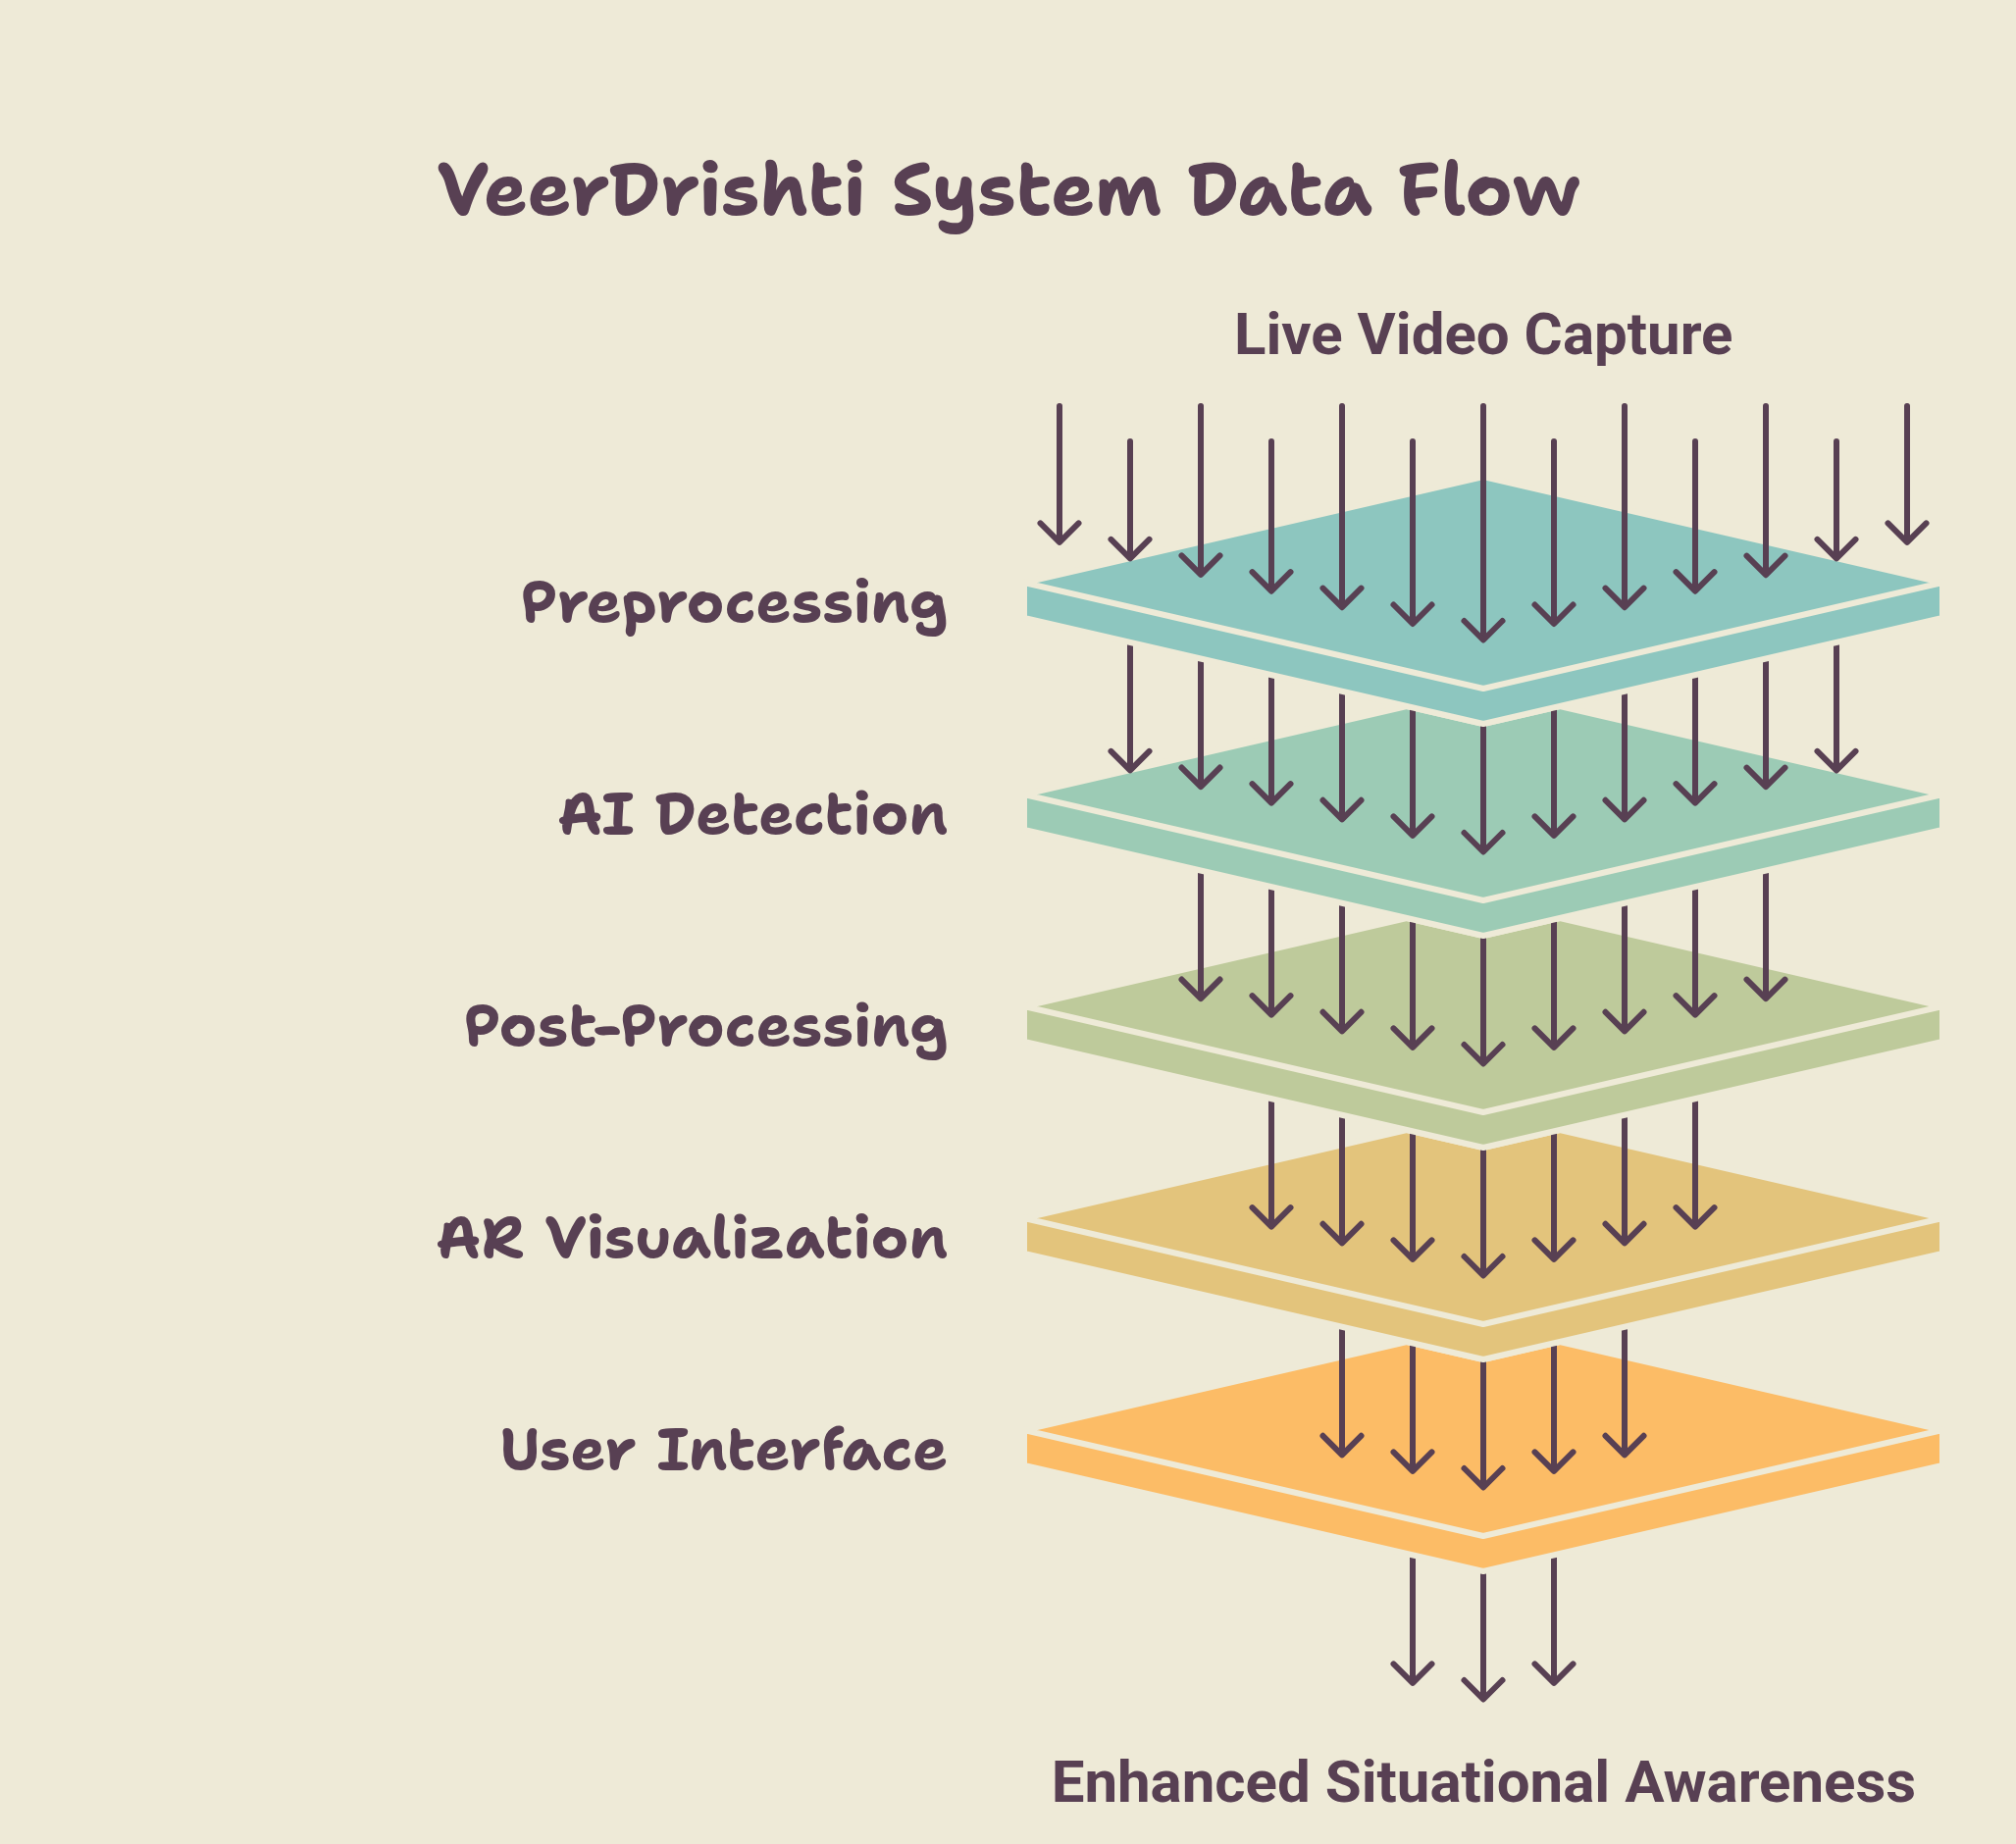
\includegraphics[width=0.62\textwidth]{images/architecture.png}
  \caption{System Architecture}\label{fig:architecture}
\end{figure}

In the prototype, CameraX supplies frames, the native YOLO pipeline prepares and analyzes them,
and Flutter YOLOView renders the outputs. The design uses the term AR visualization for the
overlays; the demonstrated outputs show image-space boxes, masks, and keypoints rather than a
world-registered augmented-reality system. Logcat supports development diagnostics independently
of the visual pipeline. Persistent mission storage is a proposed extension, not a demonstrated
layer of the current implementation.

\label{end:architecture}
\section{System Workflow}\label{sec:workflow}
Figure~\ref{fig:workflow} presents the operational workflow. The sequence
starts with RGB camera input and proceeds through preprocessing, model execution,
post-processing, user-interface visualization, and interpretation of the displayed output.

\begin{figure}[htbp]
  \centering
  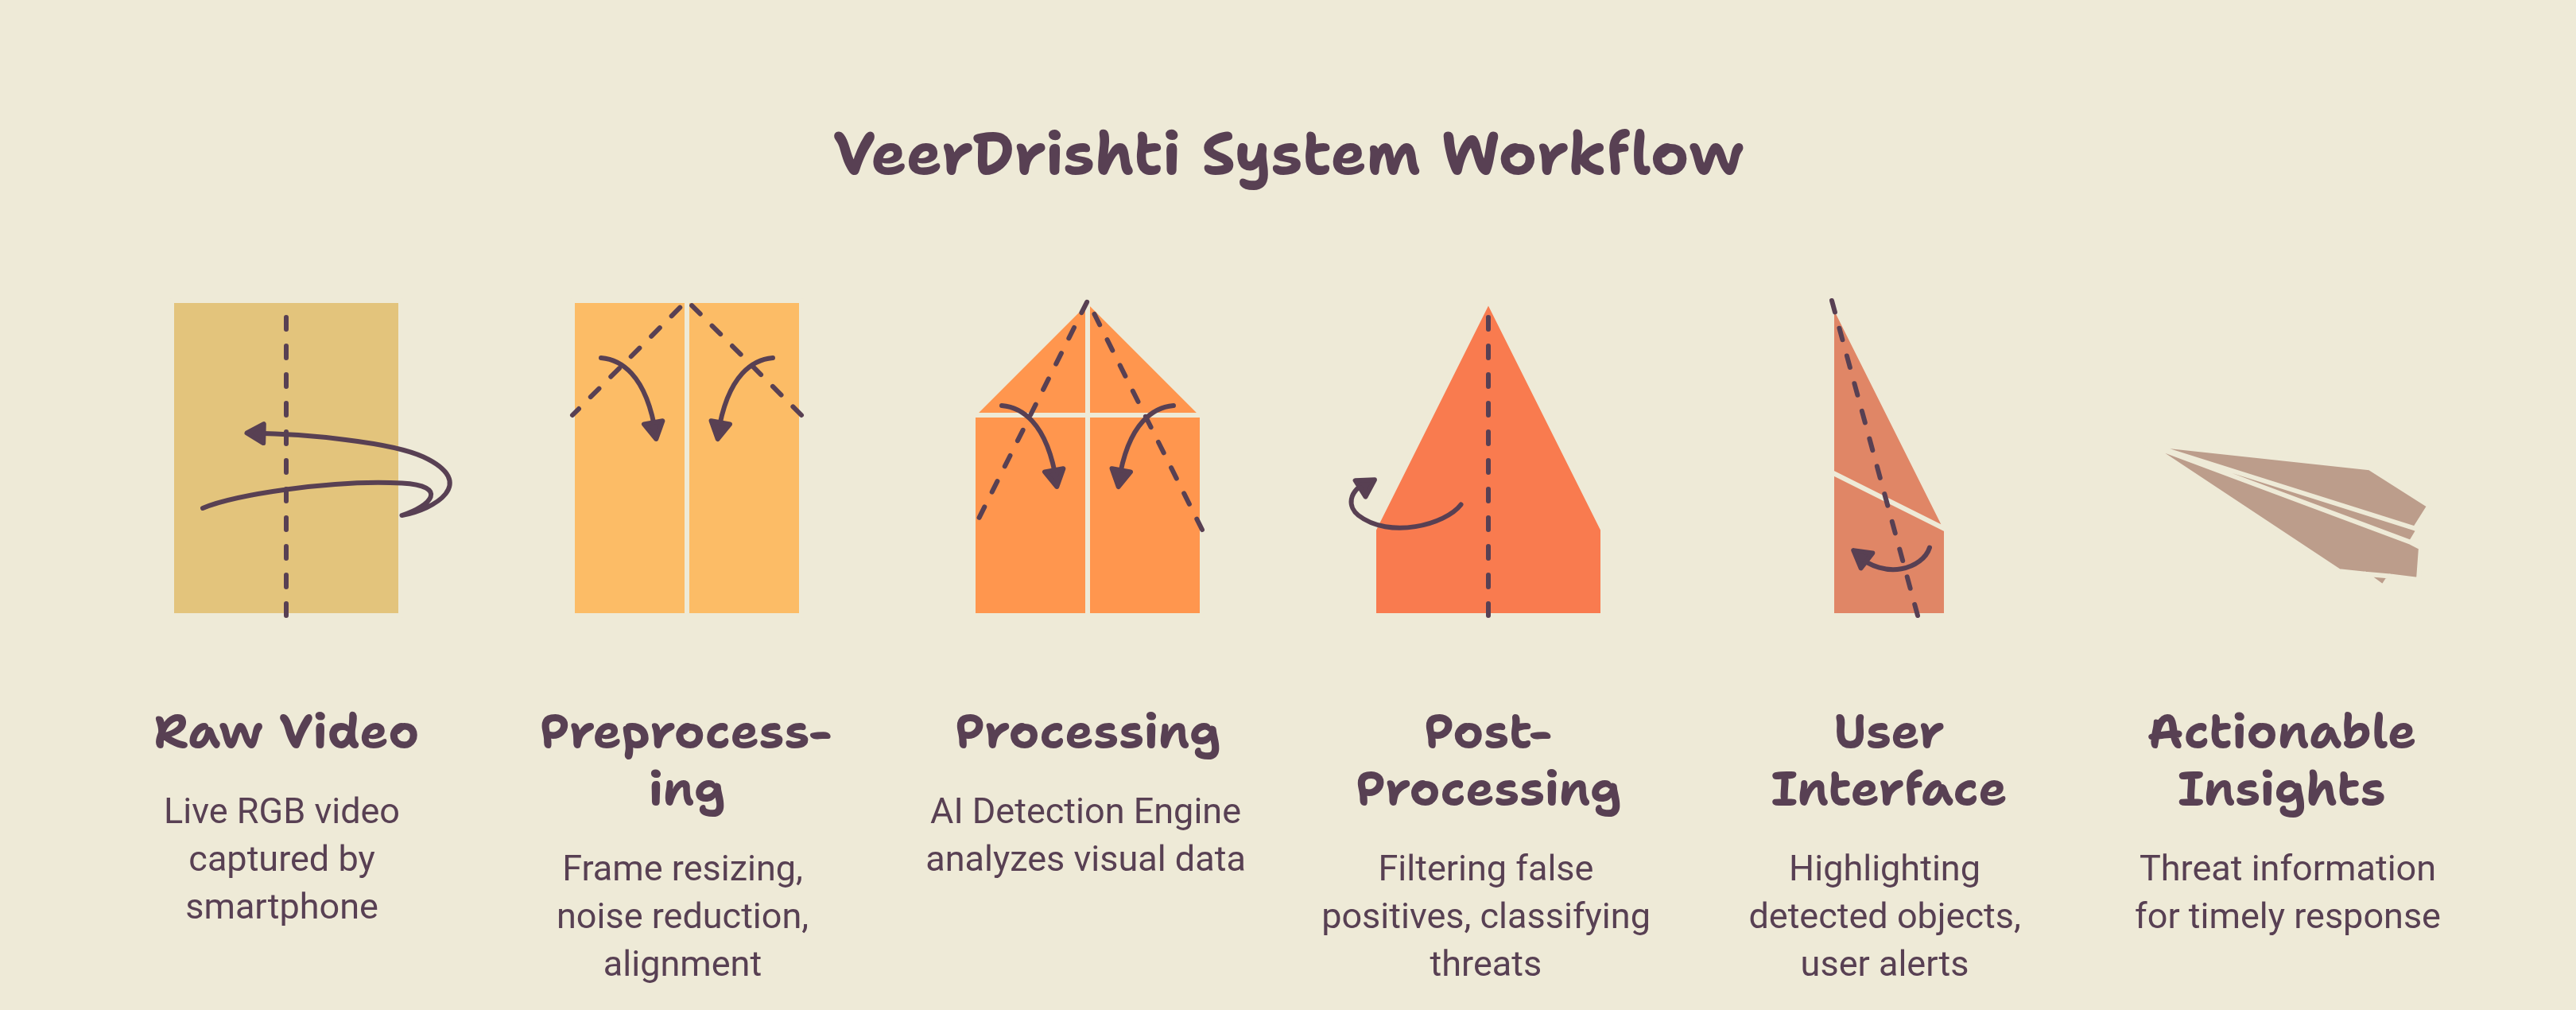
\includegraphics[width=\textwidth]{images/workflow.png}
  \caption{System Workflow}\label{fig:workflow}
\end{figure}

The implemented preprocessing operations are rotation, resizing or letterboxing, RGB conversion,
and tensor preparation. After inference, filtering settings and coordinate mapping determine
which outputs are drawn on the preview. The detection, segmentation, and pose modes provide
different visual representations within this loop. The diagram's references to threat
classification and user alerts express the wider design objective; the demonstrated outputs
establish object-class overlays and do not demonstrate hostile-intent classification or a
separate alerting service.
\label{end:workflow}\label{end:design}
\par\endgroup

  \chapter{SCHEDULING}\label{ch:scheduling}

\section{Gantt Chart}\label{sec:gantt}
The development schedule spans July--November 2026. It organizes prototype planning,
implementation, interface testing, custom model fine-tuning, model testing, final refinements,
and report drafting. The planned sequence is shown in Figure~\ref{fig:gantt} in the report's editable Gantt
format. Week positions are planning estimates rather than exact start and finish dates.

\begin{figure}[htbp]
  \centering
  \begin{ganttchart}[
    hgrid,
    vgrid,
    x unit=0.55\linewidth/16,
    title height=1
  ]{1}{20}
    \gantttitle{July}{4}
    \gantttitle{August}{4}
    \gantttitle{September}{4}
    \gantttitle{October}{4}
    \gantttitle{November}{4} \\
    \foreach \x in {1,...,5} {
      \gantttitlelist{1,...,4}{1}
    } \\
    \ganttbar[bar/.style={fill=violet!66,draw=black}]{Prototype Planning}{3}{4} \\
    \ganttbar[bar/.style={fill=blue!66,draw=black}]{Prototype Implementation}{5}{6} \\
    \ganttbar[bar/.style={fill=green!66,draw=black}]{UI Implementation}{7}{8} \\
    \ganttbar[bar/.style={fill=yellow!66,draw=black}]{UI Testing}{9}{9} \\
    \ganttbar[bar/.style={fill=orange!66,draw=black}]{Model Fine-Tuning}{10}{14} \\
    \ganttbar[bar/.style={fill=red!66,draw=black}]{Model Testing}{15}{15} \\
    \ganttbar[bar/.style={fill=cyan!66,draw=black}]{Final Refinements}{16}{17} \\
    \ganttbar[bar/.style={fill=gray!66,draw=black}]{Report Drafting}{18}{19}
  \end{ganttchart}
  \caption{Gantt Chart for Major Project}\label{fig:gantt}
\end{figure}

The schedule is a development plan, not evidence that every later task has been completed. The
academic year of the final submission is \AcademicYear, and the development months shown here
retain the planned 2026 dates.

\label{end:gantt}
\section{Month-wise Progress}\label{sec:progress}

\subsection{July}
The plan begins with prototype planning in the latter part of July. This stage establishes the
mobile processing pipeline and prepares the transition from the earlier literature and design
work to an Android implementation.

\subsection{August}
Prototype implementation and UI implementation occupy August in the schedule. The September
demonstration provides evidence of an integrated camera view, model outputs, task
controls, and visual overlays following these development activities.

\subsection{September}
The schedule places UI testing near the start of September, followed by custom model fine-tuning.
The available demonstration includes prototype screenshots but does not provide a completed
custom-training run or validation metrics.

\subsection{October}
The plan continues fine-tuning into October, followed by model testing and final refinements.
Completion of these tasks should be documented with the model configuration, training records,
test data, and measurements produced during implementation.

\subsection{November}
Final refinements and report drafting extend into November. The final report consolidates the
implementation details, evaluated results, limitations, and conclusions. Planned tasks are
to be updated with actual progress before submission.
\label{end:progress}\label{end:scheduling}

  \chapter{IMPLEMENTATION}\label{ch:implementation}
\begingroup\emergencystretch=3em

\section{Prototype Overview}\label{sec:prototype}
VeerDrishti is implemented as an Android application that combines a live camera feed with
on-device computer-vision inference. The implementation uses Android CameraX for video capture,
Ultralytics YOLO26 Nano and its variants for inference, Flutter for the interface, and Android
Logcat for development diagnostics. The prototype brings these components together to display
detections directly over the camera view.

The implementation focuses on the capture--inference--visualization loop. The prototype demonstrates
ordinary object detection, segmentation overlays, and human pose visualization. The longer-term
combat-vision objective guides the application, but thermal fusion, open-vocabulary recognition,
combat-specific fine-tuning, and persistent mission recording are separate extensions whose
completion is not established by the current prototype evidence.

\label{end:prototype}
\section{Module Implementation}\label{sec:modules}

\subsection{Input Module}
Android CameraX provides the live camera input. The application exposes the camera view through
the Flutter interface so that users can observe the scene and its associated overlays together.
The portrait and landscape screenshots demonstrate operation in both orientations. Camera access
requires Android camera permission; denial or interruption must be handled before attempting to
run the inference pipeline.

\subsection{Preprocessing Module}
Preprocessing is handled by the native YOLO inference pipeline. This stage includes frame rotation,
resizing or letterboxing, RGB conversion, and input tensor
preparation. Rotation keeps the analyzed image consistent with device orientation. Resizing and
letterboxing adapt the camera frame to the model input while preserving the information needed
to align output coordinates with the preview. The exact input resolution and normalization
settings depend on the deployed model configuration and should be recorded for reproducibility.

\subsection{Inference Module}
YOLO26 Nano and its task variants form the inference component. Computation takes
place on the device, supporting a prototype that does not require a remote server for each frame.
The interface exposes Det, Seg, and Pose modes, corresponding to detection, segmentation, and pose
outputs. The precise model export format, class configuration, and hardware execution delegate
must be taken from the application configuration when documenting a reproducible deployment.

\subsection{Post-Processing Module}
The native inference output is passed to the Flutter YOLOView integration for display. The
application renders bounding boxes, class labels, and confidence information on the live camera
feed. Segmentation mode adds colored object-region overlays, while pose mode displays body
keypoints and their connecting lines. Detection coordinates must be mapped to the displayed
preview after rotation, letterboxing, scaling, or zoom so that the overlays remain aligned with
the visible objects.

\subsection{User Interface Module}
Flutter supplies the application interface, camera display, mode controls, and visual output.
The demonstration screenshots show confidence and intersection-over-union (IoU) threshold controls,
zoom information, and runtime indicators. Keeping these controls in the camera view allows users
to inspect the effect of a configuration change without switching to a separate results screen.
Object labels describe model predictions; an object or person label alone does not establish
hostile intent or distinguish a combatant from a civilian.

\subsection{Development Logging Module}
Android Logcat records runtime logs and debugging information during development and testing.
These logs support diagnosis of camera initialization, inference integration, and application
behavior. This development logging mechanism is distinct from a persistent detection-event or
mission-video archive. The current implementation does not include a demonstrated database,
encrypted recording service, or post-mission retrieval interface.

\label{end:modules}
\section{Frame Processing Pipeline}\label{sec:pipeline}
The module descriptions define the following processing sequence for the prototype:
\begin{enumerate}
  \item Initialize the selected camera and model task, then present the live preview after camera
    permission is available.
  \item Obtain an analyzable frame from CameraX and account for its orientation.
  \item Resize or letterbox the frame, convert it to RGB, and prepare the input tensor in the
    native inference pipeline.
  \item Run the selected YOLO26 Nano task variant on the device and obtain its output.
  \item Apply the configured filtering settings and map the resulting coordinates to the preview.
  \item Render labels, boxes, masks, or pose keypoints through YOLOView, display runtime
    information, and continue with subsequent frames.
    \label{end:pipeline}
\end{enumerate}

\section{Interface and Detection Controls}\label{sec:controls}
The demonstration screenshots show a confidence threshold of 0.25 and an IoU threshold of 0.70.
The confidence setting controls the minimum score accepted for display. The IoU setting controls
overlap filtering where the selected model pipeline uses it. Changing either threshold can alter
the visible output, so evaluation runs should record both values along with the selected task and
model. The implementation record should state whether all task variants use the same suppression mechanism.

The interface also displays frames per second and processing times, including preprocessing,
inference, and post-processing components. These values help inspect responsiveness during a
demonstration. They are displayed runtime observations, not a substitute for repeated timing
measurements on a documented device. Chapter~\ref{ch:result} records the displayed values and
distinguishes them from a sustained-performance benchmark.

\label{end:controls}
\section{Integration and Testing}\label{sec:integration}
Integration testing connects camera capture, model execution, and overlay rendering as one
application workflow. The demonstrated exhibits involve scissors, a mouse, furniture, laptops,
bottles, and groups of people. These scenes exercise multiple visible objects and the three task
modes. Portrait and landscape exhibits also provide evidence for checking preview
orientation and output alignment.

For reproducible testing, record the Android device and version, application build, model file,
task mode, input resolution, thresholds, and execution backend. Separate functional checks from
accuracy and performance evaluation: a correctly rendered box verifies an interface path, while
precision, recall, mAP, and sustained frame rate require defined data and measurement procedures.
The available prototype material supports an initial functional demonstration; the Result chapter describes
the available observations and the evaluation details still needed.
\label{end:integration}\label{end:implementation}
\par\endgroup

  \chapter{RESULT}\label{ch:result}

\section{Demonstration Setup}\label{sec:demonstration}
The results in this chapter are based on the demonstrated Android prototype. The available
evidence consists of application screenshots in indoor settings, showing everyday objects and
groups of people. The screenshots display a confidence threshold of 0.25 and an IoU threshold of
0.70, together with task controls and runtime readings.

These exhibits document the prototype's visible behavior. The available material does not identify
the device model, annotated test-set size, model input resolution, execution backend, or timing
sample duration. Consequently, the reported values are transcriptions of displayed readings, and
the visual demonstrations are not presented as a controlled accuracy benchmark.

\label{end:demonstration}
\section{Visual Output}\label{sec:visual}

\subsection{Detection, Segmentation, and Pose Modes}
Figure~\ref{fig:result-modes} presents three portrait demonstrations. The detection exhibit labels
scissors with a displayed score of 94.2. The segmentation exhibit shows colored regions and labels
for ordinary indoor objects. The pose exhibit combines person boxes with connected body keypoints
in a group scene. Together, these outputs demonstrate that the application can present distinct
computer-vision tasks through the same camera interface.

\begin{figure}[htbp]
  \centering
  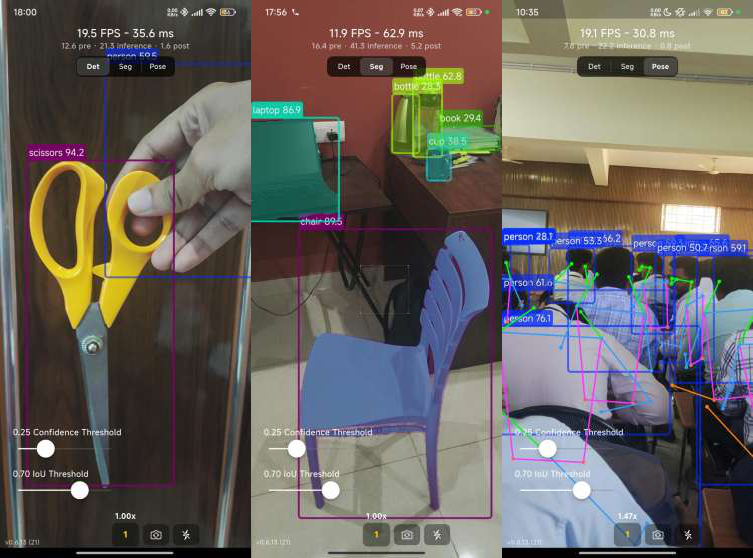
\includegraphics[width=\textwidth]{images/result-modes.png}
  \caption[Detection, Segmentation, and Pose]{Detection, segmentation, and pose outputs from the
    demonstrated prototype.}
  \label{fig:result-modes}
\end{figure}

\subsection{Landscape Object Detection}
The tabletop exhibit in Figure~\ref{fig:result-tabletop} displays a mouse and scissors with scores
of 95.2 and 92.9 respectively. The boxes correspond to the visible objects in the landscape view.
These values are model confidence scores for the displayed predictions; they are not percentages
of correct detections over a test dataset.

\begin{figure}[htbp]
  \centering
  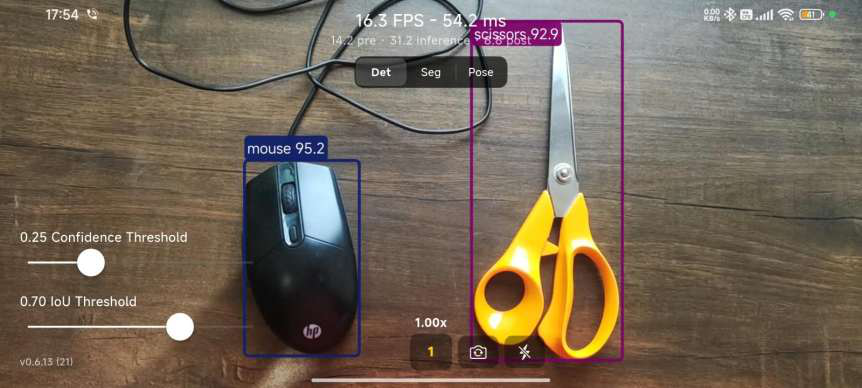
\includegraphics[width=\textwidth]{images/result-tabletop.png}
  \caption[Landscape Object Detection]{Landscape object-detection output from the demonstrated
    prototype.}
  \label{fig:result-tabletop}
\end{figure}

\subsection{Segmentation and Group Pose Visualization}
Figure~\ref{fig:result-interior} shows the interior scene. The screenshot includes region overlays
and labels for a couch, vase, laptop, and bottle. The displayed bottle score is 28.6, which is
above the configured 25\% confidence threshold but substantially lower than the laptop score of
90.3. This illustrates why per-object confidence and visual checking matter when interpreting the
output.

\begin{figure}[htbp]
  \centering
  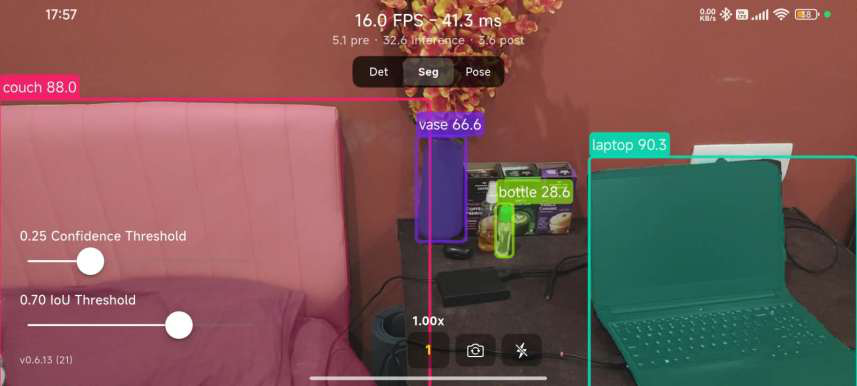
\includegraphics[width=\textwidth]{images/result-interior.png}
  \caption[Indoor Segmentation Output]{Indoor segmentation output from the demonstrated prototype.}
  \label{fig:result-interior}
\end{figure}

The group scene in Figure~\ref{fig:result-pose} contains multiple person boxes and connected pose
keypoints, including partially occluded subjects. This establishes that multi-person overlays were
displayed in the demonstrated scene. It does not quantify pose accuracy, tracking consistency, or
performance under battlefield conditions.

\begin{figure}[htbp]
  \centering
  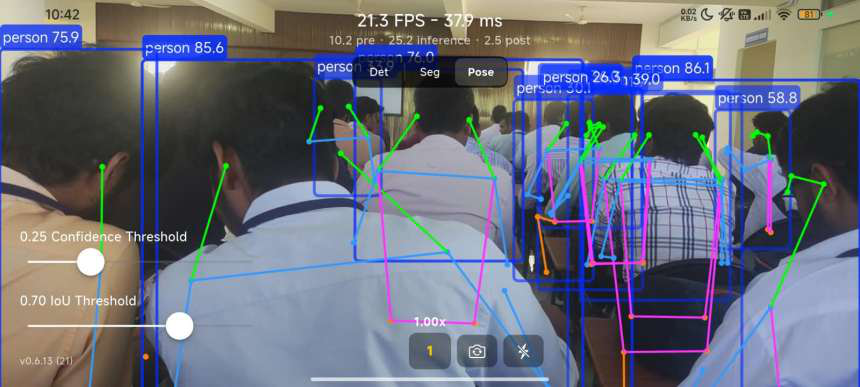
\includegraphics[width=\textwidth]{images/result-pose.png}
  \caption[Multi-Person Pose Output]{Multi-person pose output from the demonstrated prototype.}
  \label{fig:result-pose}\label{end:visual}
\end{figure}

% Finish the visual evidence before discussing the numerical readings.
\clearpage
\section{Displayed Runtime Measurements}\label{sec:runtime}
Table~\ref{tab:runtime} records the frame-rate and processing-time readings visible in the six
exhibits. The values span 11.9--21.3 FPS and 30.8--62.9 ms of displayed processing time. They
refer to different scenes and task modes, so they should not be treated as an average over one
uniform experiment or used to rank model variants without additional test controls.

\begin{table}[htbp]
  \centering
  \caption{Displayed Runtime Readings}\label{tab:runtime}
  \begin{tabular}{p{7.3cm}crr}
    \toprule
    \textbf{Exhibit} & \textbf{View} & \textbf{FPS} & \textbf{Time (ms)} \\
    \midrule
    Exhibit A: Portrait scissors detection & Portrait & 19.5 & 35.6 \\
    Exhibit B: Portrait segmentation & Portrait & 11.9 & 62.9 \\
    Exhibit C: Portrait group pose & Portrait & 19.1 & 30.8 \\
    Exhibit D: Landscape mouse and scissors & Landscape & 16.3 & 54.2 \\
    Exhibit E: Landscape interior segmentation & Landscape & 16.0 & 41.3 \\
    Exhibit F: Landscape group pose & Landscape & 21.3 & 37.9 \\
    \bottomrule
  \end{tabular}
\end{table}

The landscape segmentation screenshot decomposes its 41.3 ms reading into 5.1 ms preprocessing,
32.6 ms inference, and 3.6 ms post-processing. The group-pose screenshot similarly shows 10.2 ms,
25.2 ms, and 2.5 ms, totaling 37.9 ms. In both snapshots, inference is the largest displayed
component, making model execution an important target for further profiling.

The displayed FPS is not simply the reciprocal of the processing-time field. For instance, 37.9 ms
corresponds to approximately 26.4 processing cycles per second, whereas the screenshot reports
21.3 FPS. Capture, scheduling, rendering, and the application's averaging conventions can affect
the relationship between these indicators. The timing windows are not defined, so the
processing-time field is not claimed to measure end-to-end camera-to-display latency.

\label{end:runtime}
\section{Discussion and Limitations}\label{sec:discussion}
The demonstration shows a functional foundation: live camera input, on-device inference,
task-specific visualization, configurable thresholds, and displayed runtime information. The
exhibits support continued development of a portable situational-awareness application. They also
show that the demonstrated classes are predominantly ordinary objects and people, rather than a
validated combat-specific threat vocabulary.

Quantitative accuracy evaluation requires an annotated dataset and a defined test split. Precision,
recall, and mAP are not reported for the current prototype because the available material does not
contain the necessary measurements. Similarly, sustained FPS, latency distributions, power
consumption, and thermal behavior require repeated runs on a documented device. Numerical results
reported for papers in the literature review remain results of those studies, not measurements of
VeerDrishti.

Further evaluation should cover small or distant objects, occlusion, camera motion, illumination
changes, false detections, missed detections, and overlay alignment. Combat-specific fine-tuning,
thermal fusion, open-vocabulary recognition, and persistent event storage should be documented
with their own implementation and evaluation evidence when completed. The current results
therefore establish demonstrated prototype behavior while leaving robustness and operational
effectiveness to be assessed through controlled testing.
\label{end:discussion}\label{end:result}

  \chapter{CONCLUSION}\label{ch:conclusion}
\begingroup\emergencystretch=3em
\noindent VeerDrishti has progressed from a proposed combat-vision framework to an Android prototype that
connects camera capture, on-device inference, and visual output. The demonstration identifies
CameraX, YOLO26 Nano task variants, Flutter YOLOView, and Logcat as the
main implementation components. The presented screenshots demonstrate object detection,
segmentation, and multi-person pose overlays in portrait and landscape views, with configurable
thresholds and runtime indicators. This establishes the application's capture-to-display
foundation and provides concrete evidence for the Implementation and Result chapters.

The observed runtime readings and visual exhibits do not establish battlefield accuracy,
sustained performance, or a reduction in casualties. Those outcomes remain project objectives
that require combat-relevant data and controlled evaluation. The next development steps are to
document the deployed configuration, evaluate accuracy and latency on repeatable test cases,
refine the interface, and validate the selected model for the intended object classes. Thermal
fusion, open-vocabulary recognition, and persistent event recording remain possible extensions
rather than demonstrated features. By grounding further development in measured evidence,
VeerDrishti can advance toward a more reliable, portable visual decision-support system.
\label{end:conclusion}
\par\endgroup

  \clearpage
  \defbibheading{bibintoc}[REFERENCES]{%
    \section*{#1}\addcontentsline{toc}{chapter}{#1}\label{ch:references}}
  \begingroup
    \emergencystretch=2em
    \printbibliography[heading=bibintoc,title={REFERENCES}]
    \label{end:references}
  \endgroup
  % Submission material follows the references and precedes the appendices.
  \clearpage
\phantomsection
\label{submission:icstim}
\thispagestyle{report}
\section*{ICSTIM 2026 ABSTRACT SUBMISSION}
The following page reproduces the abstract submitted for ICSTIM 2026, the
International Conference on Sustainable Technologies, Innovation and Management.
The paper was suggested for submission under the title \emph{“VeerDrishti: A Computer Vision Framework for Real-Time Situational Awareness and
Visual Threat Assessment.”}

\begin{center}
  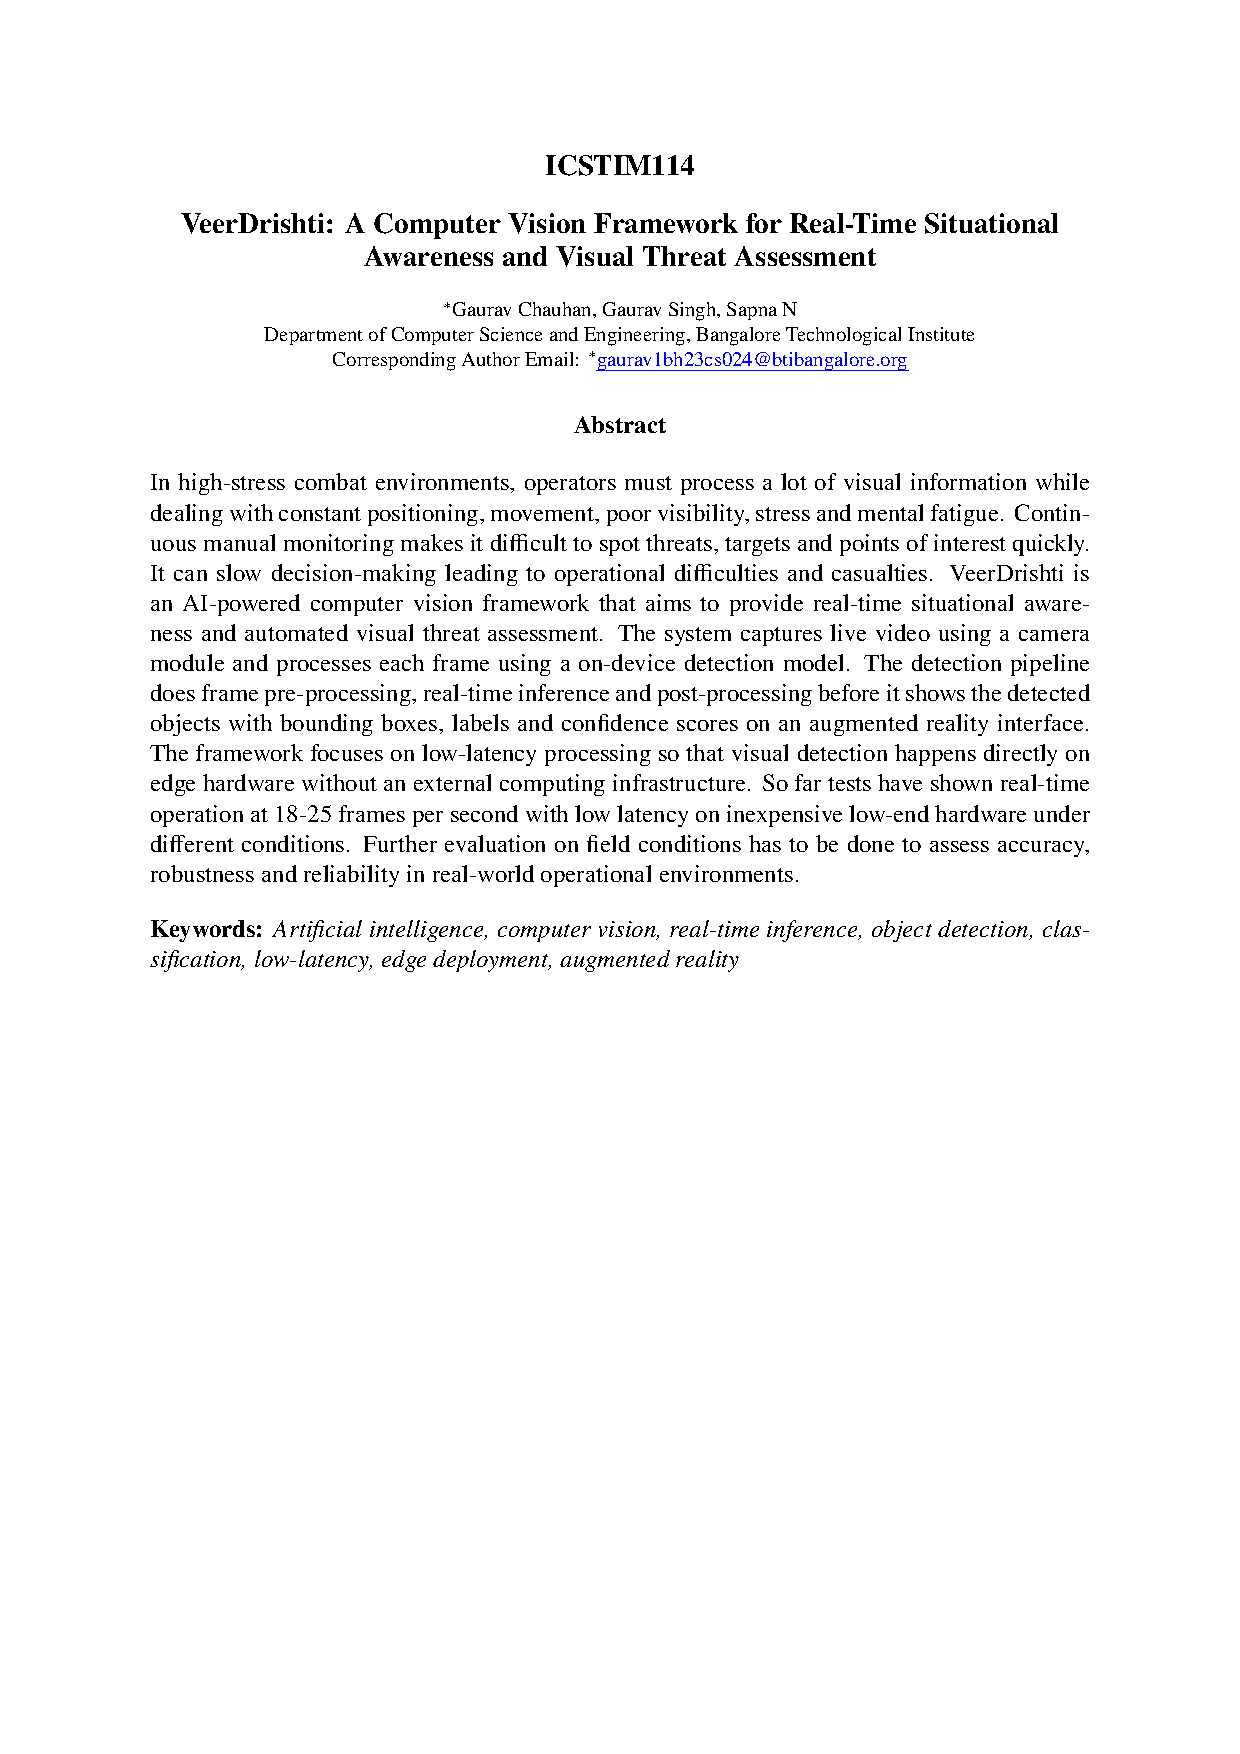
\includegraphics[page=1,width=.86\textwidth,height=.72\textheight,keepaspectratio]{B3 - Abstract.pdf}
\end{center}

\clearpage
\phantomsection
\label{submission:drdo}
\thispagestyle{report}
\section*{DRDO SYNOPSIS SUBMISSION}
The following page reproduces the synopsis mailed to the DRDO Students
Development Program executive. The response is awaited.

\begin{center}
  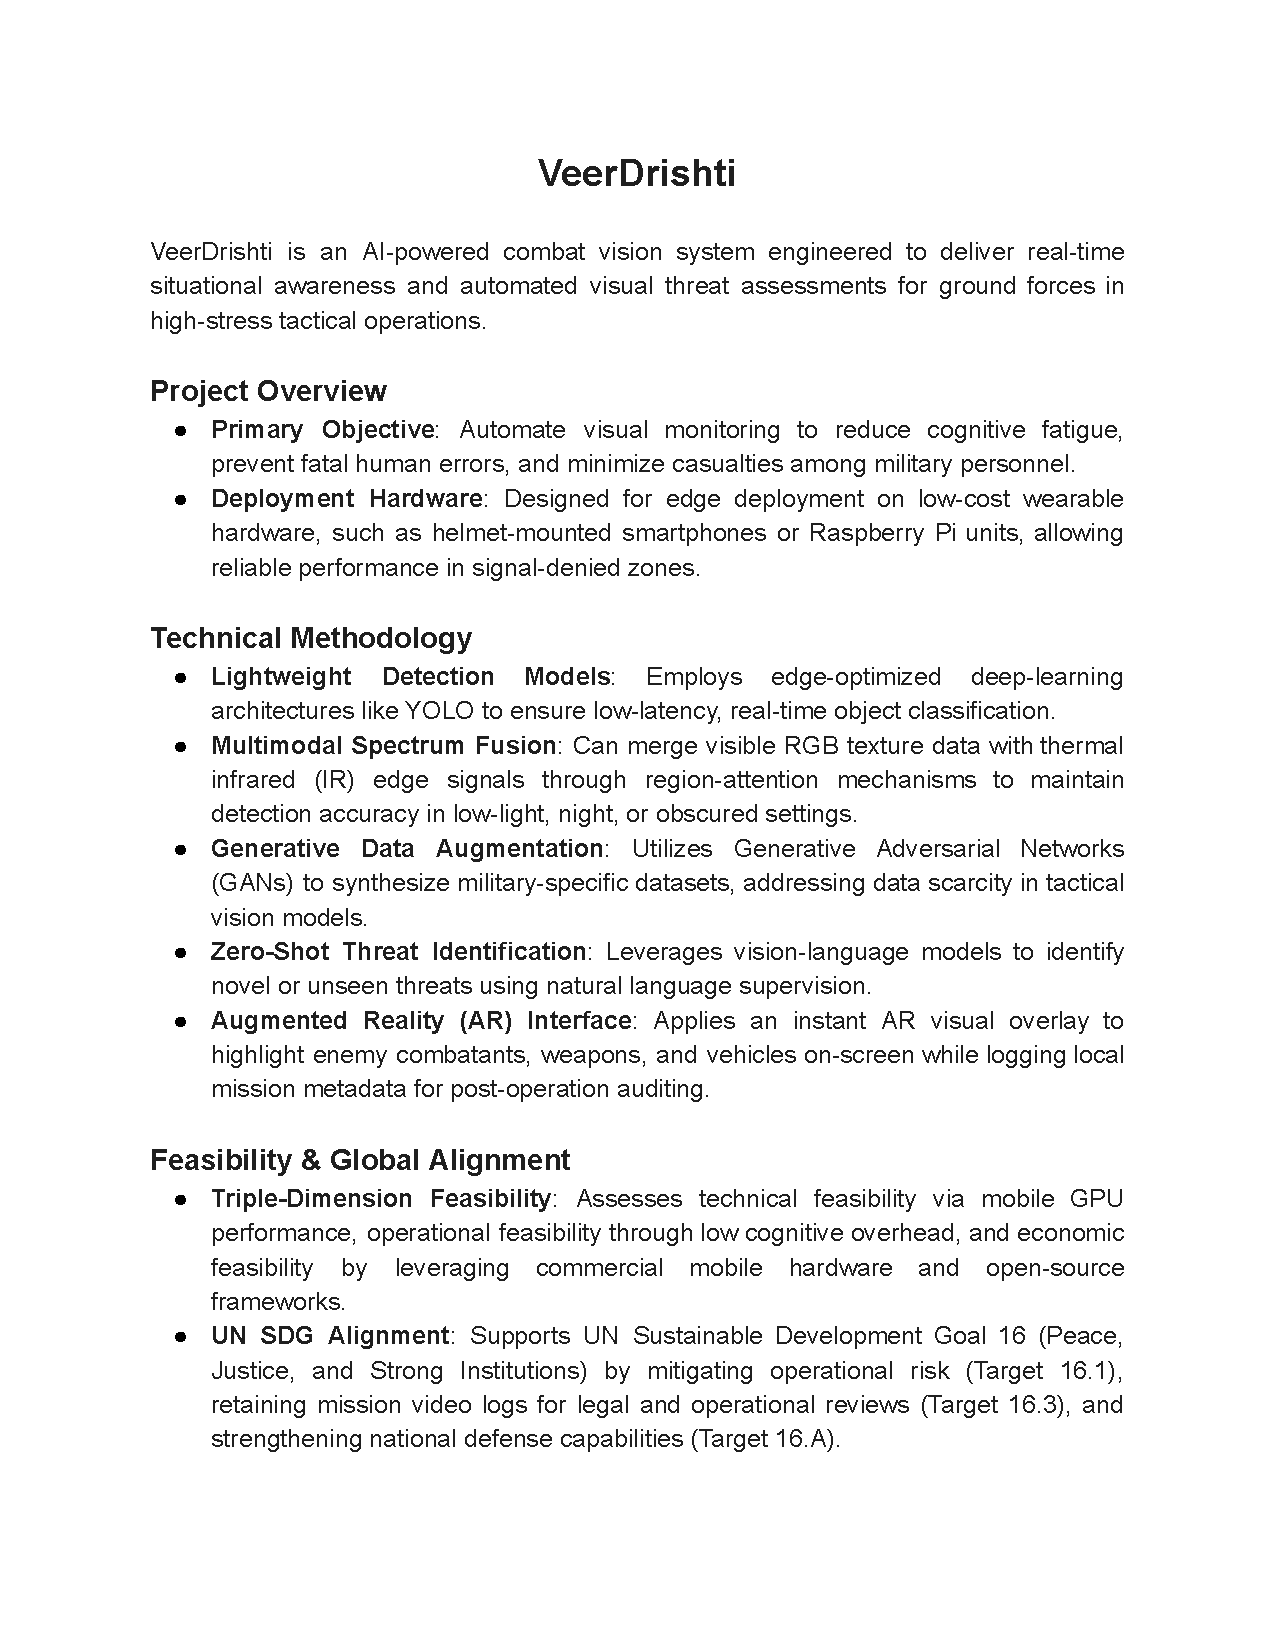
\includegraphics[page=1,width=.86\textwidth,height=.75\textheight,keepaspectratio]{Synopsis.pdf}
\end{center}

  % Appendices follow the references and use alphabetic appendix numbering.
  \appendix
  \renewcommand{\chaptername}{Appendix}
  \chapter*{APPENDIX A}
\phantomsection
\label{appendix:a}

\begin{center}
  \textbf{SOURCE CODE LISTING (1/3)}
\end{center}
\begingroup
\fontsize{6.5pt}{6.8pt}\selectfont
\begin{verbatim}
// Ultralytics YOLO Android wrapper
// AGPL-3.0 License - https://ultralytics.com/license
package com.ultralytics.yolo

import android.content.Context
import android.graphics.*
import android.net.Uri
import android.provider.MediaStore
import android.util.Log
import androidx.camera.core.ImageProxy
import kotlinx.coroutines.*
import java.io.IOException
import java.net.URL
class YOLO(
    private val context: Context,
    private val modelPath: String,
    val task: YOLOTask,
    private val labels: List<String> = emptyList(),
    private val useGpu: Boolean = true,
    private var numItemsThreshold: Int = 30,
    private val classifierOptions: Map<String, Any>? = null
) {
    private val tag = "YOLO"
    private var closed = false
    private val predictorDelegate = lazy(LazyThreadSafetyMode.NONE) {
        Predictor.create(context, modelPath, task, labels, useGpu,
            numItemsThreshold, classifierOptions) as BasePredictor
    }
    private val predictor: BasePredictor
        get() { check(!closed); return predictorDelegate.value }
    @Synchronized
    fun predict(bitmap: Bitmap, rotateForCamera: Boolean = false): YOLOResult {
        predictor.includeRawMaskData = true
        val result = predictor.predict(bitmap, bitmap.width, bitmap.height,
            rotateForCamera, isLandscape = false)
        return result.copy(originalImage = bitmap,
            annotatedImage = drawAnnotations(bitmap, result, rotateForCamera),
            accelerator = predictor.accelerator)
    }
    @Synchronized
    fun predict(imageProxy: ImageProxy): YOLOResult? {
        val bitmap = ImageUtils.toBitmap(imageProxy) ?: return null
        val rotation = imageProxy.imageInfo.rotationDegrees
        predictor.cameraRotationDegrees = rotation
        val result = predictor.predict(bitmap, imageProxy.width, imageProxy.height, true, false)
        return result.copy(originalImage = bitmap,
            annotatedImage = drawAnnotations(bitmap, result, true, rotation),
            accelerator = predictor.accelerator)
    }
    @Synchronized
    fun predict(imageUri: Uri): YOLOResult? = try {
        val bitmap = MediaStore.Images.Media.getBitmap(context.contentResolver, imageUri)
        predict(bitmap)
    } catch (error: IOException) {
        Log.e(tag, "Failed to load Uri: ${error.message}"); null
    }
    suspend fun predict(imageUrl: String): YOLOResult? = withContext(Dispatchers.IO) {
        try {
            val bitmap = BitmapFactory.decodeStream(URL(imageUrl).openStream())
            predict(bitmap)
        } catch (error: IOException) {
            Log.e(tag, "Failed to load URL: ${error.message}"); null
        }
    }
\end{verbatim}
\endgroup

\clearpage
\begin{center}
  \textbf{SOURCE CODE LISTING (2/3)}
\end{center}
\begingroup
\fontsize{6.5pt}{6.8pt}\selectfont
\begin{verbatim}
    private fun calculateSmartLabelRect(
        box: RectF, labelWidth: Float, labelHeight: Float,
        viewWidth: Float, viewHeight: Float
    ): RectF {
        var left = box.left; var top = box.top - labelHeight
        var right = left + labelWidth; var bottom = box.top
        if (top < 0) { top = box.top; bottom = top + labelHeight }
        if (left < 0) { left = 0f; right = labelWidth }
        if (right > viewWidth) { right = viewWidth; left = right - labelWidth }
        if (bottom > viewHeight) { bottom = viewHeight; top = bottom - labelHeight }
        return RectF(left, top, right, bottom)
    }

    private fun drawAnnotations(bitmap: Bitmap, result: YOLOResult,
        rotateForCamera: Boolean = true, rotationDegrees: Int? = null): Bitmap {
        val degrees = rotationDegrees ?: 90
        val rotated = degrees % 180 != 0
        val output = if (rotateForCamera) Bitmap.createBitmap(
            if (rotated) bitmap.height else bitmap.width,
            if (rotated) bitmap.width else bitmap.height, Bitmap.Config.ARGB_8888
        ) else bitmap.copy(Bitmap.Config.ARGB_8888, true)
        val canvas = Canvas(output)
        if (rotateForCamera) { canvas.save()
            canvas.translate(output.width / 2f, output.height / 2f)
            canvas.rotate(degrees.toFloat())
            canvas.drawBitmap(bitmap, -bitmap.width / 2f, -bitmap.height / 2f, null)
            canvas.restore() }
        val paint = Paint().apply { style = Paint.Style.STROKE }
        val sx = output.width / result.origShape.width.toFloat()
        val sy = output.height / result.origShape.height.toFloat()
        fun scale(box: RectF) = RectF(box.left * sx, box.top * sy,
            box.right * sx, box.bottom * sy)

        when (task) {
            YOLOTask.DETECT, YOLOTask.SEGMENT, YOLOTask.POSE -> {
                result.boxes.forEach { box ->
                    paint.color = ultralyticsColors[box.index % ultralyticsColors.size]
                    val bounds = scale(box.xywh)
                    canvas.drawRoundRect(bounds, 12f, 12f, paint)
                    val text = "${box.cls} ${(box.conf * 100).toInt()}%"
                    val label = calculateSmartLabelRect(bounds,
                        paint.measureText(text) + 16f, 48f,
                        output.width.toFloat(), output.height.toFloat())
                    paint.style = Paint.Style.FILL
                    canvas.drawRoundRect(label, 12f, 12f, paint)
                    paint.color = Color.WHITE; canvas.drawText(text,
                        label.left + 8f, label.bottom - 8f, paint)
                    paint.style = Paint.Style.STROKE
                }
                // Full implementation also draws masks, keypoints, and skeletons.
            }
            YOLOTask.SEMANTIC, YOLOTask.DEPTH -> {
                result.semanticMask?.let { drawMask(canvas, it, output) }
                result.depthMap?.let { drawDepth(canvas, it, output) }
            }
            YOLOTask.CLASSIFY -> drawTopFive(canvas, result, paint)
            YOLOTask.OBB -> drawOrientedBoxes(canvas, result, paint, sx, sy)
        }
        return output
    }

    @Synchronized fun setConfidenceThreshold(value: Double) =
        predictor.setConfidenceThreshold(value)
    @Synchronized fun setIouThreshold(value: Double) = predictor.setIouThreshold(value)
    @Synchronized fun setNumItemsThreshold(max: Int) {
        numItemsThreshold = max; predictor.setNumItemsThreshold(max)
    }
    fun getConfidenceThreshold(): Float = predictor.getConfidenceThreshold().toFloat()
    fun getIouThreshold(): Float = predictor.getIouThreshold().toFloat()
    @Synchronized fun close() {
        closed = true
        if (predictorDelegate.isInitialized()) predictorDelegate.value.close()
    }
}
\end{verbatim}
\endgroup

\clearpage
\begin{center}
  \textbf{SOURCE CODE LISTING (3/3)}
\end{center}
\begingroup
\fontsize{6.5pt}{6.8pt}\selectfont
\begin{verbatim}
    private fun drawMask(canvas: Canvas, mask: Bitmap, output: Bitmap) {
        val paint = Paint(Paint.ANTI_ALIAS_FLAG).apply {
            alpha = 96
            xfermode = PorterDuffXfermode(PorterDuff.Mode.SRC_OVER)
        }
        val scaled = Bitmap.createScaledBitmap(mask, output.width,
            output.height, true)
        canvas.drawBitmap(scaled, 0f, 0f, paint)
    }

    private fun drawDepth(canvas: Canvas, depth: Bitmap, output: Bitmap) {
        val paint = Paint(Paint.ANTI_ALIAS_FLAG)
        val scaled = Bitmap.createScaledBitmap(depth, output.width,
            output.height, true)
        paint.colorFilter = ColorMatrixColorFilter(ColorMatrix(floatArrayOf(
            1f, 0f, 0f, 0f, 0f, 0f, 1f, 0f, 0f, 0f,
            0f, 0f, 1f, 0f, 0f, 0f, 0f, 0f, 1f, 0f)))
        canvas.drawBitmap(scaled, 0f, 0f, paint)
    }

    private fun drawTopFive(canvas: Canvas, result: YOLOResult, paint: Paint) {
        result.topClassifications.take(5).forEachIndexed { index, item ->
            val y = 48f + index * 42f
            paint.style = Paint.Style.FILL
            paint.color = Color.WHITE
            paint.textSize = 28f
            canvas.drawText("${item.label}: ${item.confidence}", 24f, y, paint)
        }
    }

    private fun drawOrientedBoxes(canvas: Canvas, result: YOLOResult,
        paint: Paint, sx: Float, sy: Float) {
        result.boxes.forEach { box ->
            paint.style = Paint.Style.STROKE
            paint.strokeWidth = 4f
            paint.color = ultralyticsColors[box.index % ultralyticsColors.size]
            val points = box.corners.map { PointF(it.x * sx, it.y * sy) }
            if (points.size >= 4) {
                val path = Path().apply {
                    moveTo(points[0].x, points[0].y)
                    points.drop(1).forEach { lineTo(it.x, it.y) }
                    close()
                }
                canvas.drawPath(path, paint)
            }
        }
    }

    data class DetectionSettings(
        val confidence: Float = 0.25f,
        val iou: Float = 0.45f,
        val maximumItems: Int = 30,
        val useGpu: Boolean = true
    )

    fun applySettings(settings: DetectionSettings) {
        setConfidenceThreshold(settings.confidence.toDouble())
        setIouThreshold(settings.iou.toDouble())
        setNumItemsThreshold(settings.maximumItems)
    }
\end{verbatim}
\endgroup

\label{appendix:a-end}

  \chapter*{APPENDIX B}
\phantomsection
\label{appendix:b}

\begin{center}
  \textbf{PROJECT PHOTOGRAPHS}

  \vspace{8pt}
  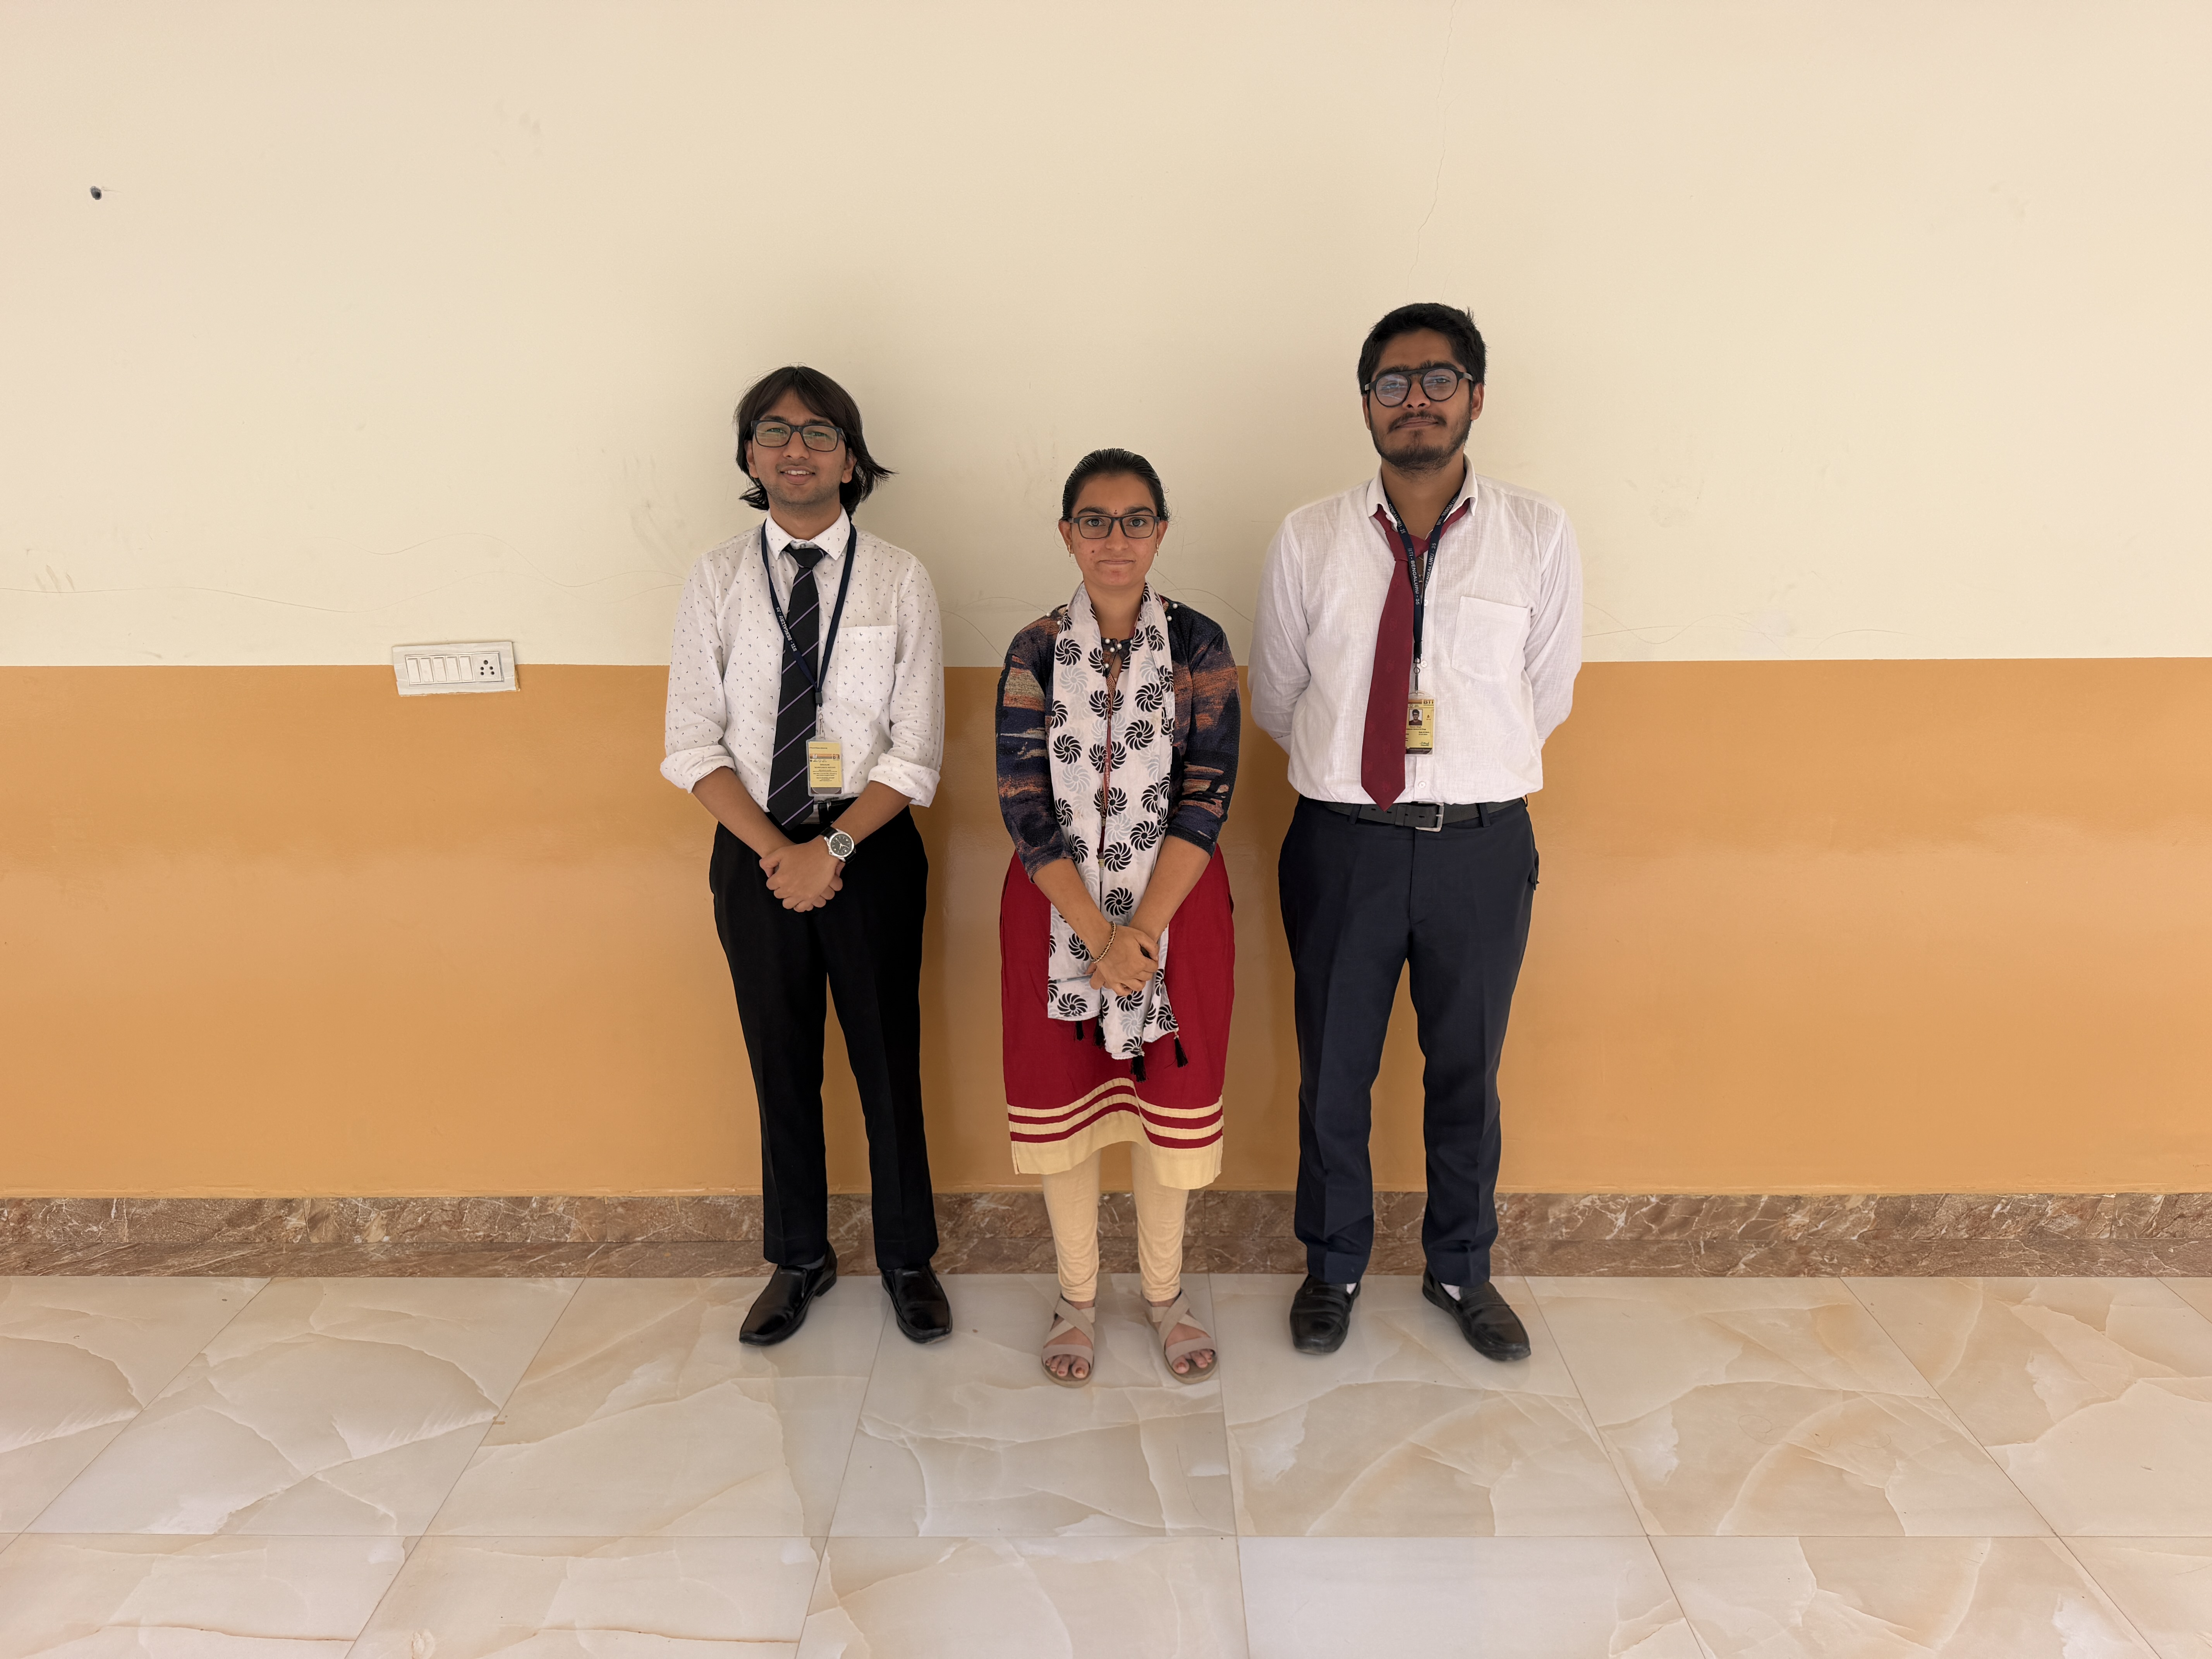
\includegraphics[width=.96\textwidth,height=.38\textheight,keepaspectratio]{images/group-guide.JPG}

  \vspace{4pt}
  \textit{Project group with the project guide}

  \vspace{12pt}
  \begin{minipage}[t]{.46\textwidth}
    \centering
    
\includegraphics[width=180pt]{images/review01-upright.jpg}

    \vspace{3pt}
    \textit{Project photograph 1}
  \end{minipage}
  \hfill
  \begin{minipage}[t]{.46\textwidth}
    \centering
    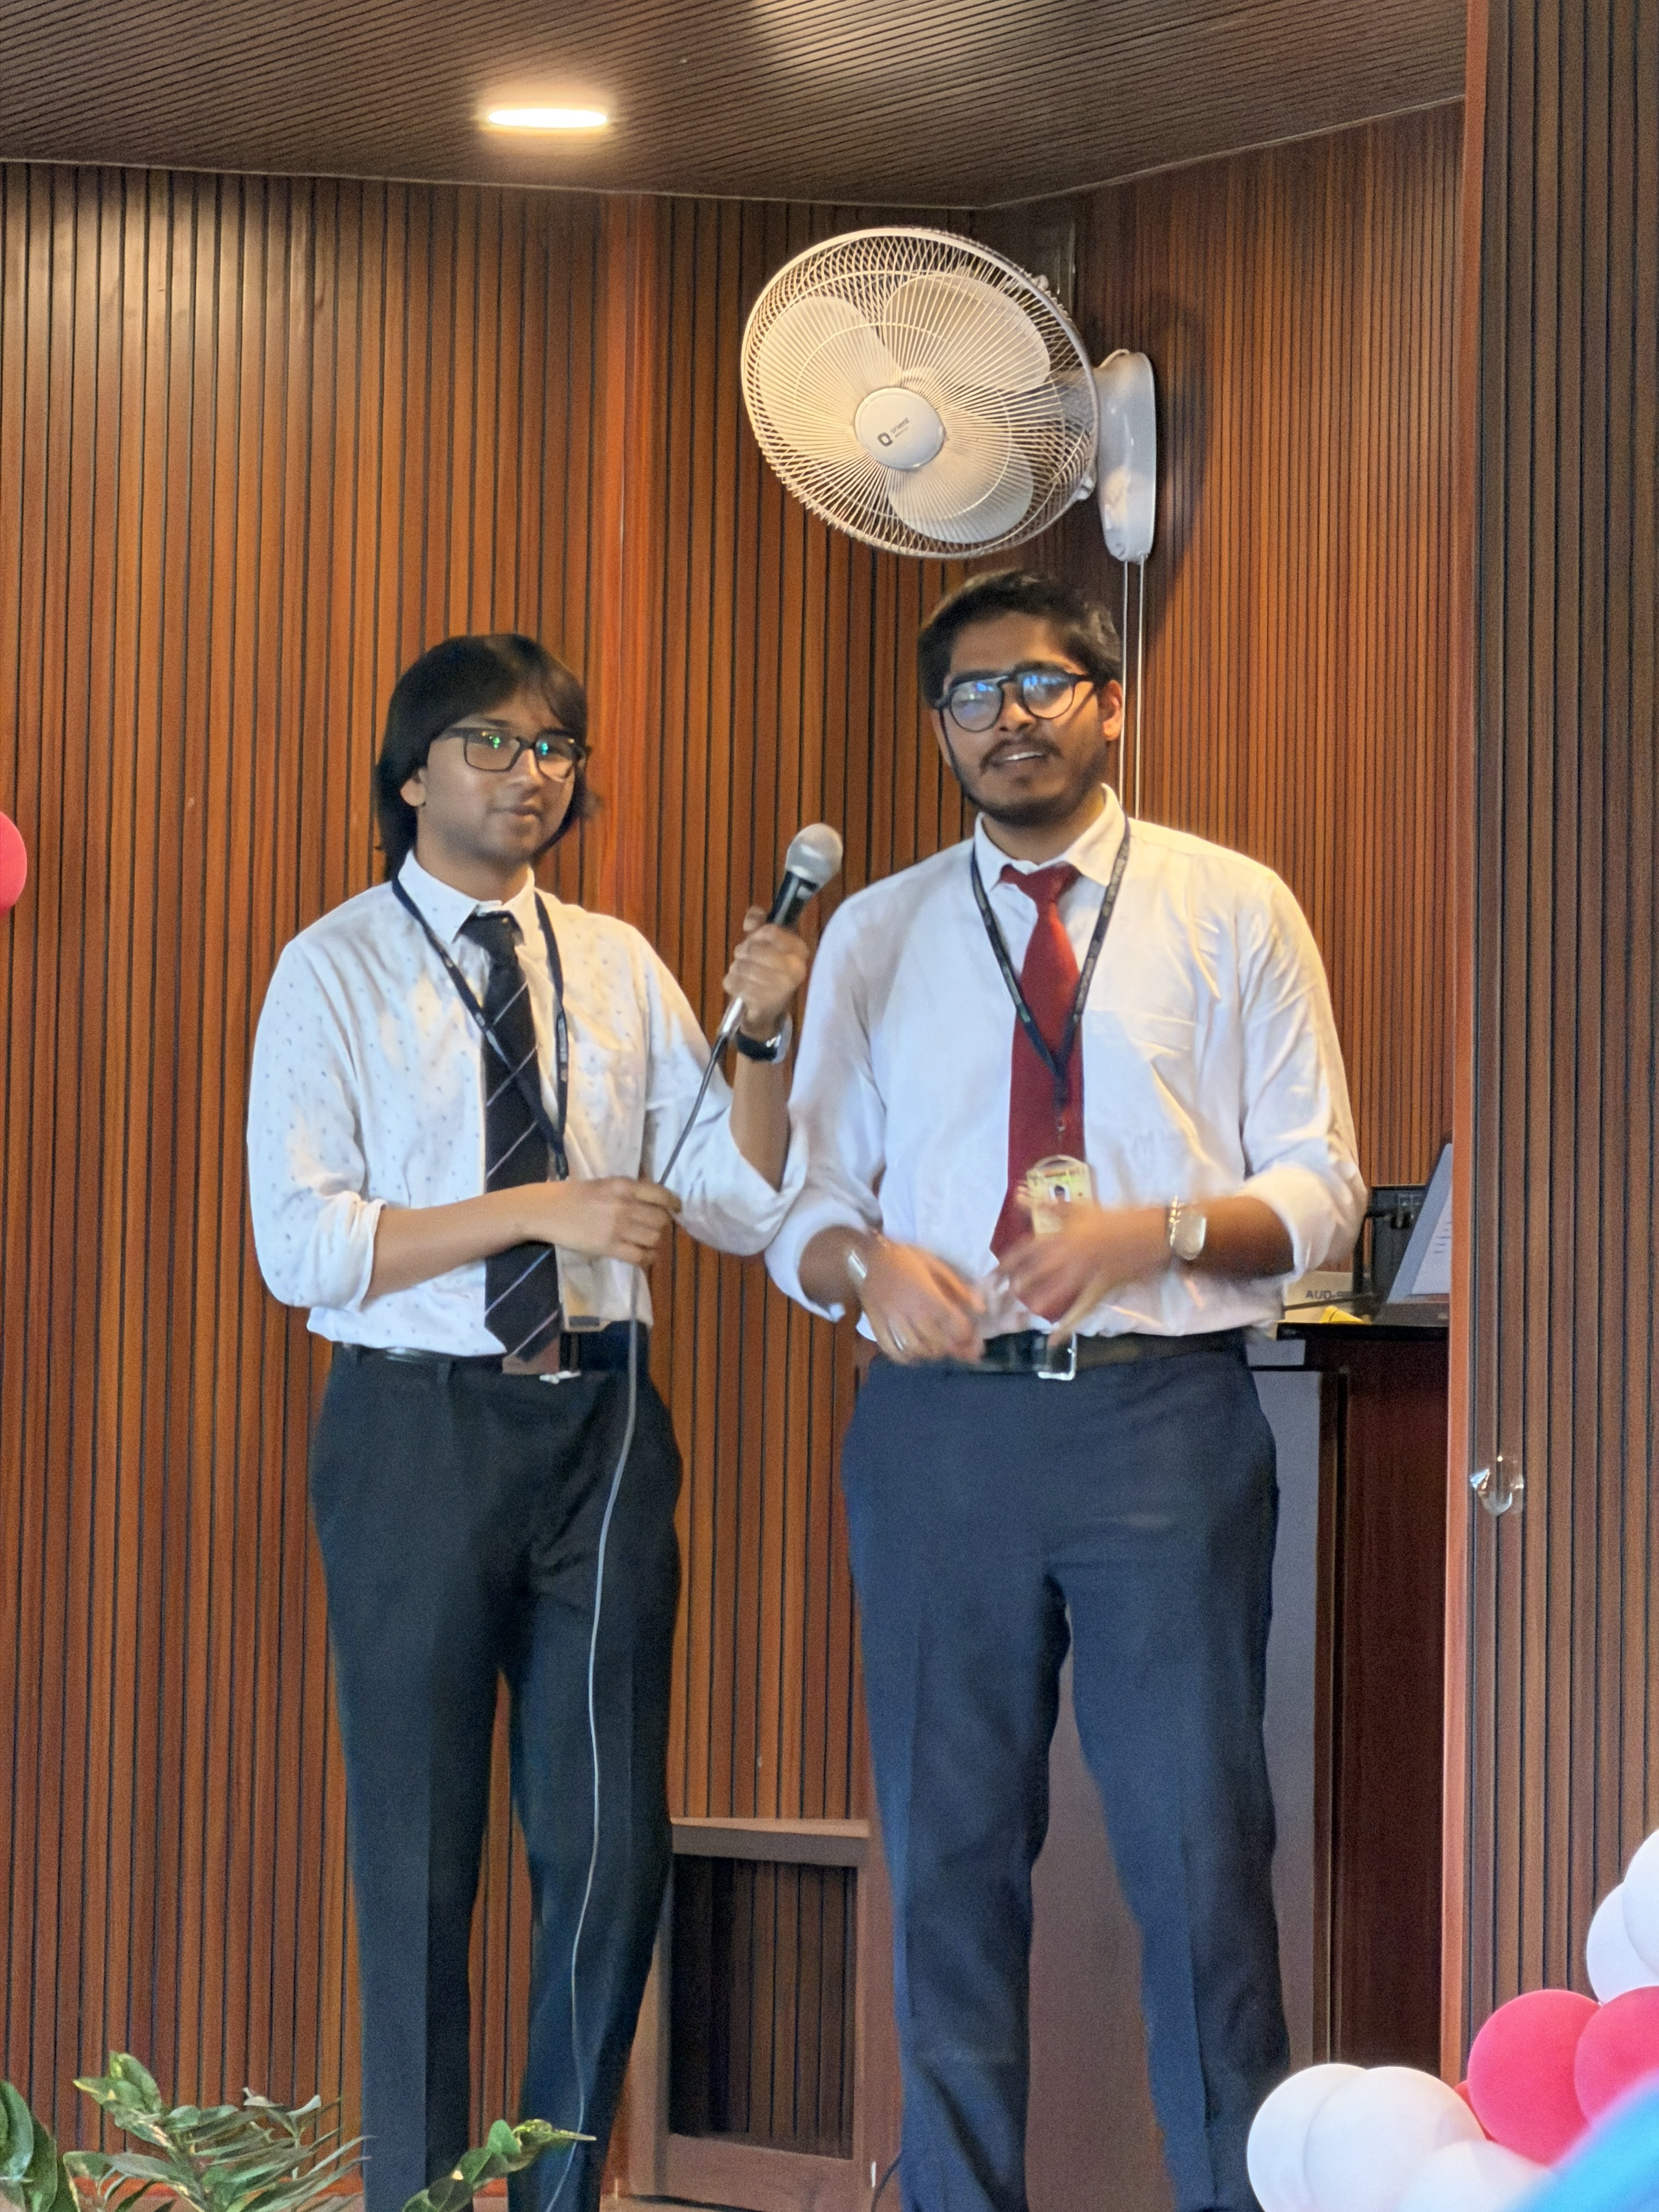
\includegraphics[width=180pt]{images/review02-upright.jpg}

    \vspace{3pt}
    \textit{Project photograph 2}
  \end{minipage}
\end{center}
\label{appendix:b-end}

\end{document}
